%%%%%%%%%%%%%%%%%%%%%%%%%%%%%%%%%%%%%%%%%
% Beamer Presentation
% LaTeX Template
% Version 1.0 (10/11/12)
%
% This template has been downloaded from:
% http://www.LaTeXTemplates.com
%
% License:
% CC BY-NC-SA 3.0 (http://creativecommons.org/licenses/by-nc-sa/3.0/)
%
%%%%%%%%%%%%%%%%%%%%%%%%%%%%%%%%%%%%%%%%%

%----------------------------------------------------------------------------------------
%   PACKAGES AND THEMES
%----------------------------------------------------------------------------------------

\documentclass[10pt]{beamer}

\mode<presentation> {

% The Beamer class comes with a number of default slide themes
% which change the colors and layouts of slides. Below this is a list
% of all the themes, uncomment each in turn to see what they look like.

\usetheme{default}
%\usetheme{AnnArbor}
%\usetheme{Antibes}
%\usetheme{Bergen}
%\usetheme{Berkeley}
%\usetheme{Berlin}
%\usetheme{Boadilla}
%\usetheme{CambridgeUS}
%\usetheme{Copenhagen}
%\usetheme{Darmstadt}
%\usetheme{Dresden}
%\usetheme{Frankfurt}
%\usetheme{Goettingen}
%\usetheme{Hannover}
%\usetheme{Ilmenau}
%\usetheme{JuanLesPins}
%\usetheme{Luebeck}
% \usetheme{Madrid}
%\usetheme{Malmoe}
%\usetheme{Marburg}
%\usetheme{Montpellier}
%\usetheme{PaloAlto}
%\usetheme{Pittsburgh}
%\usetheme{Rochester}
%\usetheme{Singapore}
%\usetheme{Szeged}
%\usetheme{Warsaw}

% As well as themes, the Beamer class has a number of color themes
% for any slide theme. Uncomment each of these in turn to see how it
% changes the colors of your current slide theme.

%\usecolortheme{albatross}
\usecolortheme{beaver}
%\usecolortheme{beetle}
%\usecolortheme{crane}
%\usecolortheme{dolphin}
%\usecolortheme{dove}
%\usecolortheme{fly}
%\usecolortheme{lily}
%\usecolortheme{orchid}
%\usecolortheme{rose}
%\usecolortheme{seagull}
%\usecolortheme{seahorse}
%\usecolortheme{whale}
%\usecolortheme{wolverine}

%\setbeamertemplate{footline} % To remove the footer line in all slides uncomment this line
\setbeamertemplate{footline}[page number] % To replace the footer line in all slides with a simple slide count uncomment this line

%\setbeamertemplate{navigation symbols}{} % To remove the navigation symbols from the bottom of all slides uncomment this line
}

\usepackage[brazil]{babel}
\usepackage[utf8]{inputenc}
\usepackage{graphicx} % Allows including images
\usepackage{booktabs} % Allows the use of \toprule, \midrule and \bottomrule in tables
\usepackage{amstext}
\usepackage{amsmath,amssymb,amsfonts,amsthm,mathtools}
\usepackage{mathrsfs}
\usepackage{bibentry}
\usepackage{algorithm, algpseudocode}
\usepackage[compatibility=false]{caption}
\usepackage{subcaption}
% \usepackage{paralist}
\usepackage{color}

\DeclareMathOperator*{\argmin}{arg\,min}
\DeclareMathOperator*{\argmax}{arg\,max}
\DeclareMathOperator*{\diag}{diag}
\DeclarePairedDelimiter\abs{\lvert}{\rvert}
\DeclarePairedDelimiter\norm{\lVert}{\rVert}

\AtBeginSection[]
{
  \begin{frame}<beamer>
    \frametitle{Seção \thesection}
    \tableofcontents[currentsection]
  \end{frame}
}

%----------------------------------------------------------------------------------------
%   TITLE PAGE
%----------------------------------------------------------------------------------------

\title[FM no problema de Coagrupamento com sobrep. de colunas]{Fatoração de Matrizes no problema de Coagrupamento com sobrepreposição de colunas}

\author{Lucas Fernandes Brunialti \\
\small{Orientadora: Profa. Dra. Sarajane Marques Peres}}
\institute[EACH USP] % Your institution as it will appear on the bottom of every slide, may be shorthand to save space
{
Escola de Artes, Ciências e Humanidades \\
Universidade de São Paulo \\ % Your institution for the title page
\medskip
\textit{lucas.brunialti@usp.br} \\
\textit{sarajane@usp.br}
}
\date{\today} % Date, can be changed to a custom date

\begin{document}

\begin{frame}
\titlepage % Print the title page as the first slide
\end{frame}

\begin{frame}
\frametitle{Agenda}
\tableofcontents
\end{frame}

%----------------------------------------------------------------------------------------
%    PRESENTATION SLIDES
%----------------------------------------------------------------------------------------

%------------------------------------------------

\section{Introdução}

% \begin{frame}
%   \frametitle{Introdução}
%   % \textcolor{red}{Porque Coagrupamento?}
%   \begin{itemize}
%     \item Agrupamento
%     \begin{itemize}
%       \item Organiza uma coleção de dados (tabela de dados por características) em grupos
%       \item Busca encontrar uma organização ``natural'' dos dados baseando-se na similaridade (ou dissimilaridade)
%       \item Existem diferentes estratégias: particional, hierárquica, baseada em densidade, etc para diversas necessidades
%       \item Descobrir quais características tornam os dados similares dentro de cada grupo é uma dessas necessidades
%       \item Uma das formas é formar grupos considerando a \textbf{similaridade parcial} ou \textbf{similaridade por partes}
%     \end{itemize}
%   \end{itemize}
%   % \textcolor{red}{Imagem da tabela}
% % \[
% % \bordermatrix{  ~    &  I_1   & \dots  &  I_m   & \dots  &  I_M   \cr
% %                U_1   & \sigma & \dots  &   ?    & \dots  & \sigma \cr
% %                \dots & \dots  & \dots  & \dots  & \dots  & \dots  \cr
% %                U_n   & \sigma & \dots  & \sigma & \dots  &   ?    \cr
% %                \dots & \dots  & \dots  & \dots  & \dots  & \dots  \cr
% %                U_N   &   ?    & \dots  & \sigma & \dots  & \sigma \cr
% %              }
% % \]
% \end{frame}

\begin{frame}
  \frametitle{Introdução}
  \begin{itemize}
    \item Agrupamento
    \begin{itemize}
      \item Coleção de dados: matriz com $n$ objetos e $m$ características
      \item Organiza uma coleção de dados em grupos
      \item Dados em um mesmo grupo são similares
      \item Estratégias: particional, hierárquica, baseada em densidade, etc
    \end{itemize}
    \item Coagrupamento
    \begin{itemize}
      \item Uma estratégia: formar grupos considerando a \textbf{similaridade parcial}, \textbf{similaridade por partes} ou \textbf{resconstrução por partes}
      \item Análises mais refinadas
      % \item Exemplo:
      % \begin{itemize}
      %   \item Aplicação de mineração de textos
      %   \item Coleção de documentos $\rightarrow$ matriz de dados
      %   \item Contagem de palavras para cada documento
      % \end{itemize}
    \end{itemize}
  \end{itemize}
  % \textcolor{red}{Imagem da tabela}
% \[
% \bordermatrix{  ~    &  I_1   & \dots  &  I_m   & \dots  &  I_M   \cr
%                U_1   & \sigma & \dots  &   ?    & \dots  & \sigma \cr
%                \dots & \dots  & \dots  & \dots  & \dots  & \dots  \cr
%                U_n   & \sigma & \dots  & \sigma & \dots  &   ?    \cr
%                \dots & \dots  & \dots  & \dots  & \dots  & \dots  \cr
%                U_N   &   ?    & \dots  & \sigma & \dots  & \sigma \cr
%              }
% \]
\end{frame}

%------------------------------------------------

\begin{frame} [shrink=15]
  \frametitle{Coagrupamento}

  \begin{figure} [htpb]
    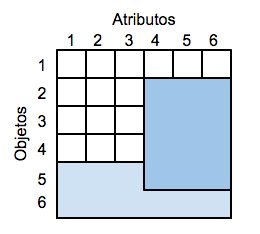
\includegraphics[width=0.8\textwidth]{img/bicluster.png}
  \end{figure}

  \begin{itemize}
    \item Visão tradicional:
    \begin{itemize}
      \item 2 cogrupos (submatrizes azul e verde)
    \end{itemize}
  \end{itemize}
\end{frame}

% \begin{frame}
%   \frametitle{Aplicação de coagrupamento de notícias}
%   % \begin{figure} [htpb]
%   %   \centering
%   %   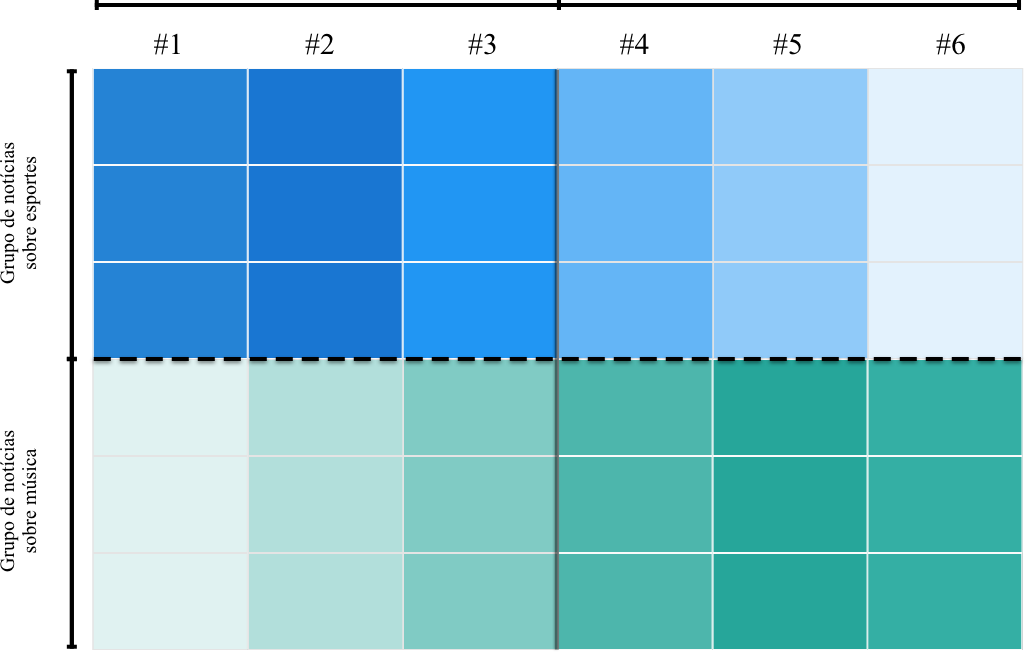
\includegraphics[scale=0.25]{img/sistema0.png}
%   % \end{figure}

%   % \begin{figure} [htpb]
%   %   \centering
%   %   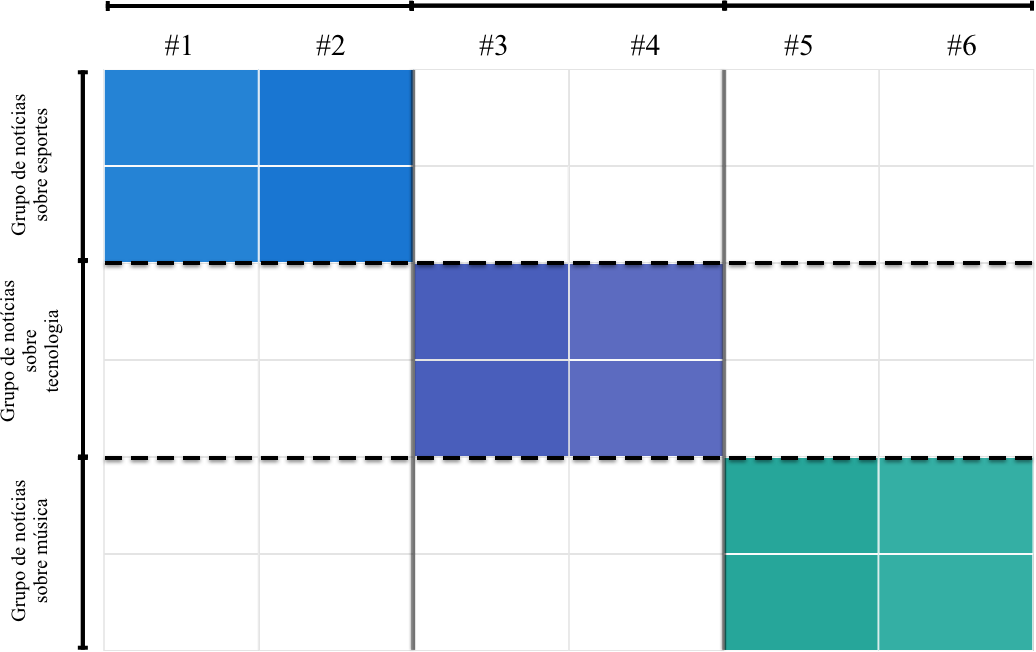
\includegraphics[scale=0.25]{img/sistema1-update.png}
%   % \end{figure}
%   \begin{itemize}
%         \item Aplicação de mineração de textos
%         \item Coleção de documentos $\rightarrow$ matriz de dados
%         \item Contagem de palavras para cada documento
%       \end{itemize}

%   \begin{figure} [htpb]
%     \centering
%     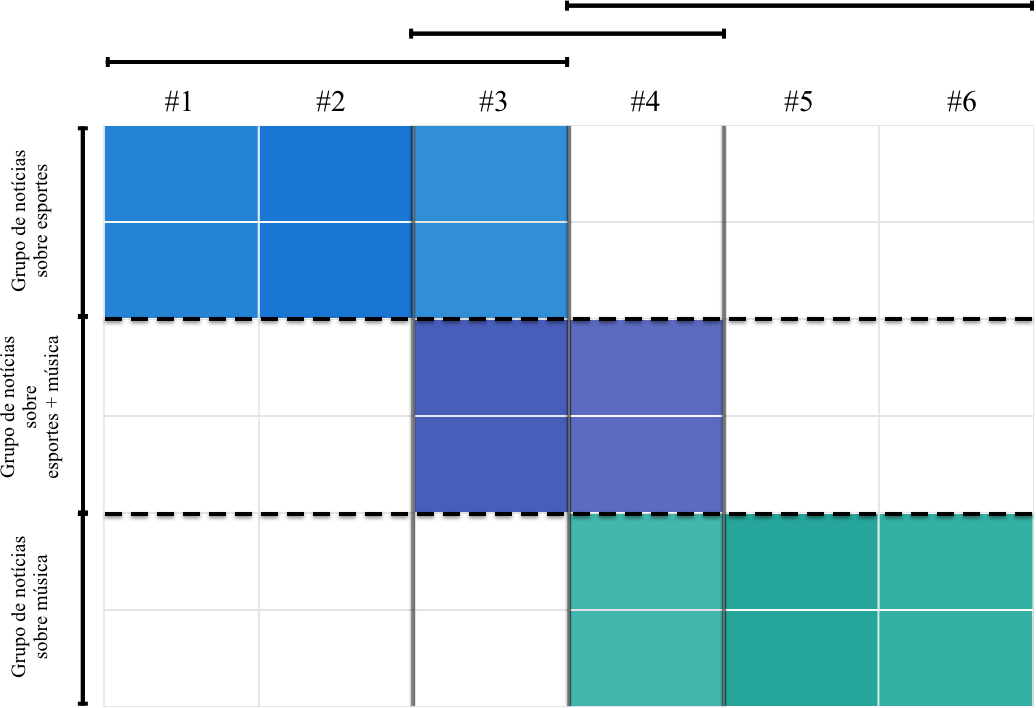
\includegraphics[scale=0.22]{img/sistema2.png}
%   \end{figure}
% \end{frame}

%------------------------------------------------

\begin{frame}
  \frametitle{Fatoração de matrizes não-negativas}
  \begin{figure}[H]
    \centering
    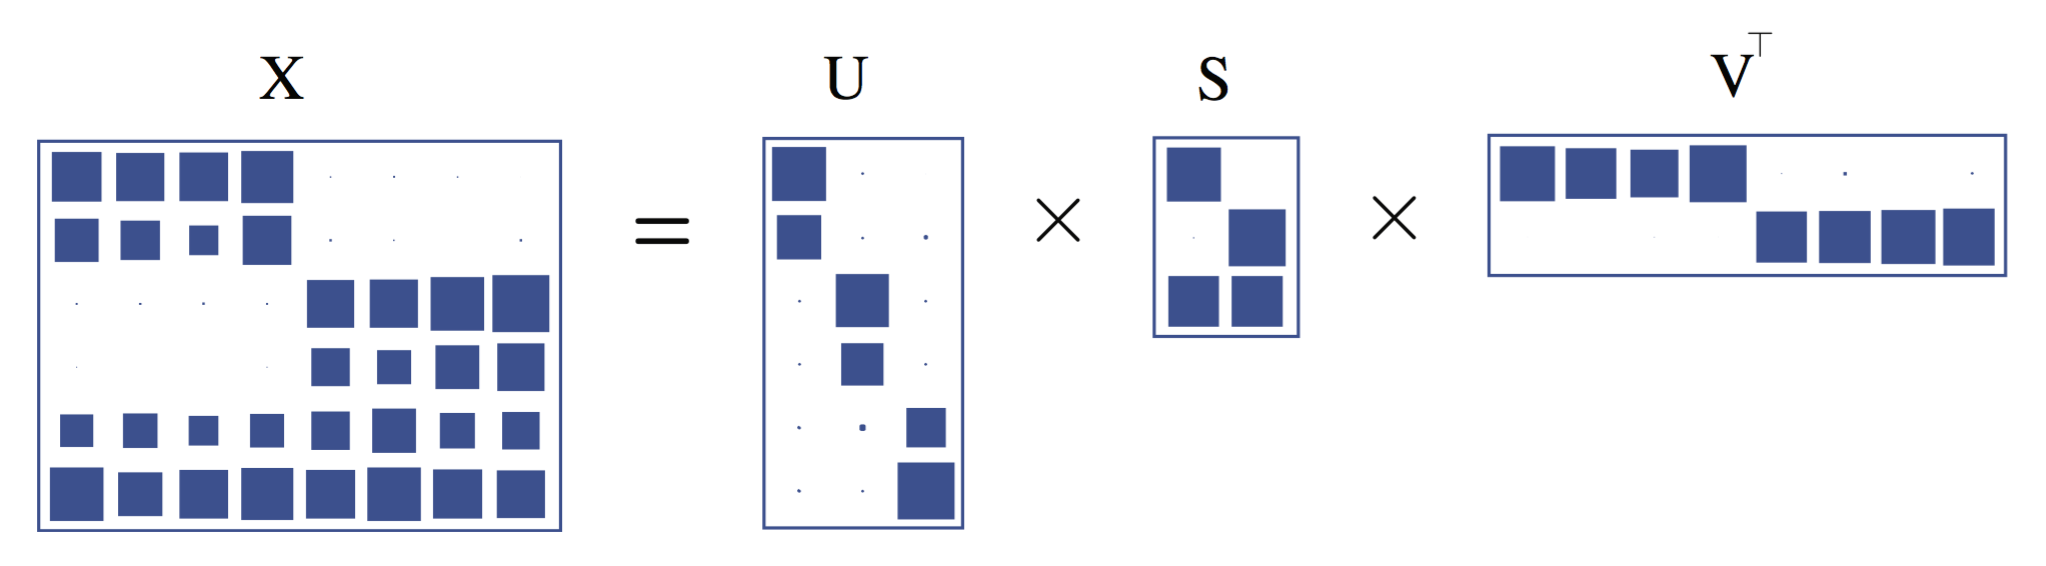
\includegraphics[width=1.0\textwidth]{img/factorizationXUSV.png}
  \end{figure}

  \begin{itemize}
    \item $U$ particionamento de linhas
    \item $V$ particionamento de colunas
    \item $S$ relação entre as partes
    \item Pós-processamento para obtenção dos cogrupos
  \end{itemize}
\end{frame}

%------------------------------------------------

\begin{frame}
  \frametitle{Estruturas de cogrupos I}

  \begin{figure}[H]
    \centering
      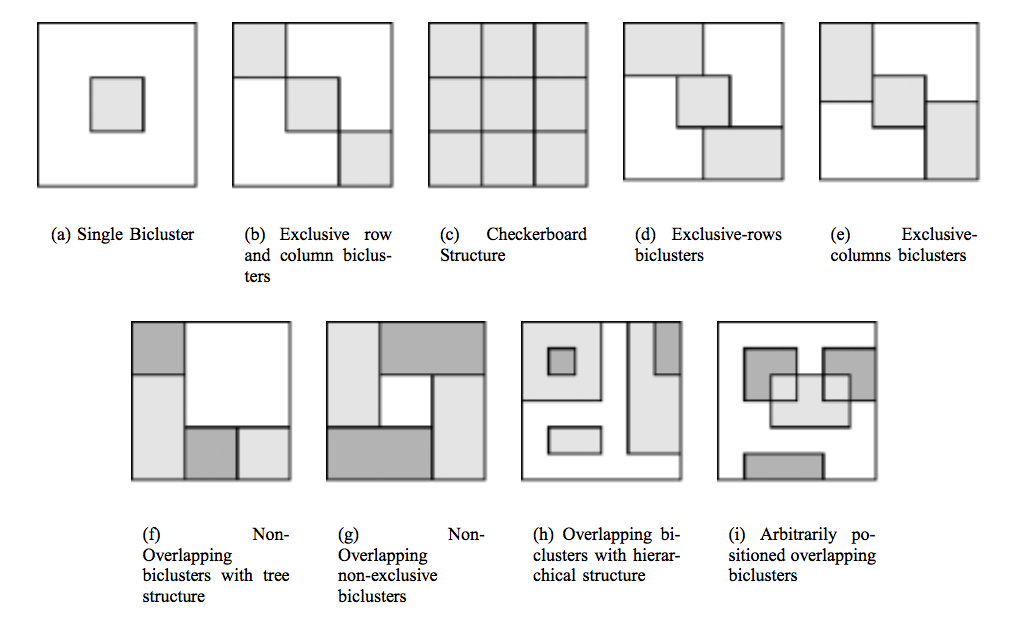
\includegraphics[width=0.8\textwidth]{img/synteticBiclusters.png}
  \end{figure}

  Estruturas de cogrupos:
  \begin{itemize}
    \item caso $3$: Coagrupamento em FM
    \item caso $4$: Coagrupamento com sobreposição de colunas em FM (proposto)
  \end{itemize}
\end{frame}

\begin{frame}
  \frametitle{Estruturas de cogrupos II}

  \begin{figure}[H]
    \centering
      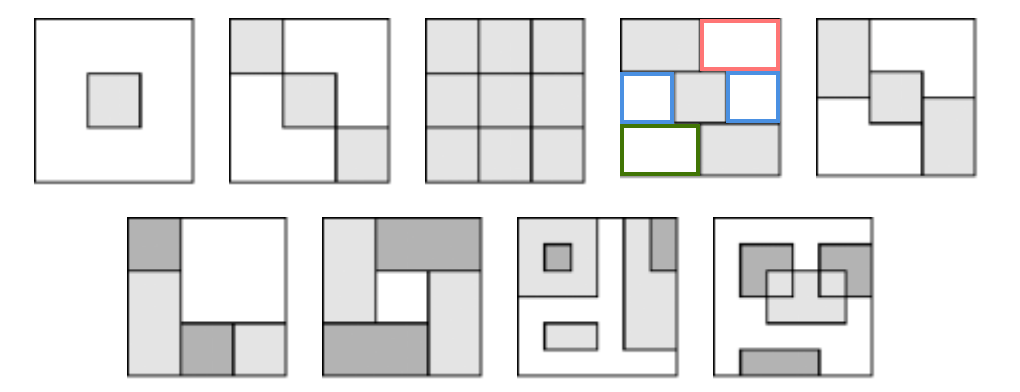
\includegraphics[width=0.8\textwidth]{img/synteticBiclusters-v2.png}
  \end{figure}

  \begin{itemize}
    \item Particionamento
  \end{itemize}
\end{frame}


\begin{frame}
  \frametitle{Aplicação de coagrupamento de notícias}
  % \begin{figure} [htpb]
  %   \centering
  %   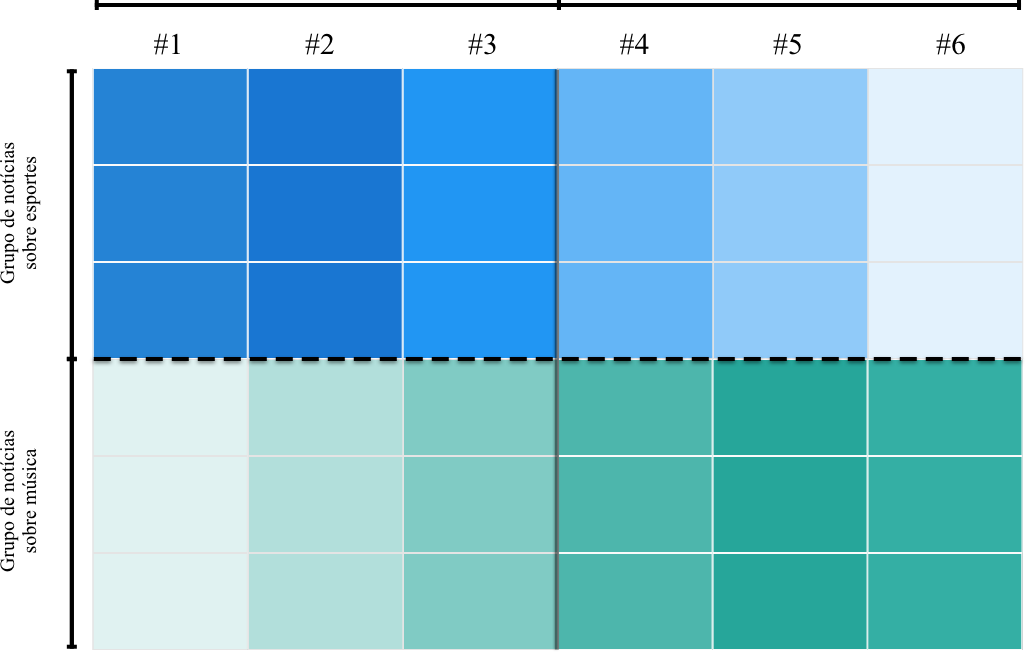
\includegraphics[scale=0.25]{img/sistema0.png}
  % \end{figure}

  % \begin{figure} [htpb]
  %   \centering
  %   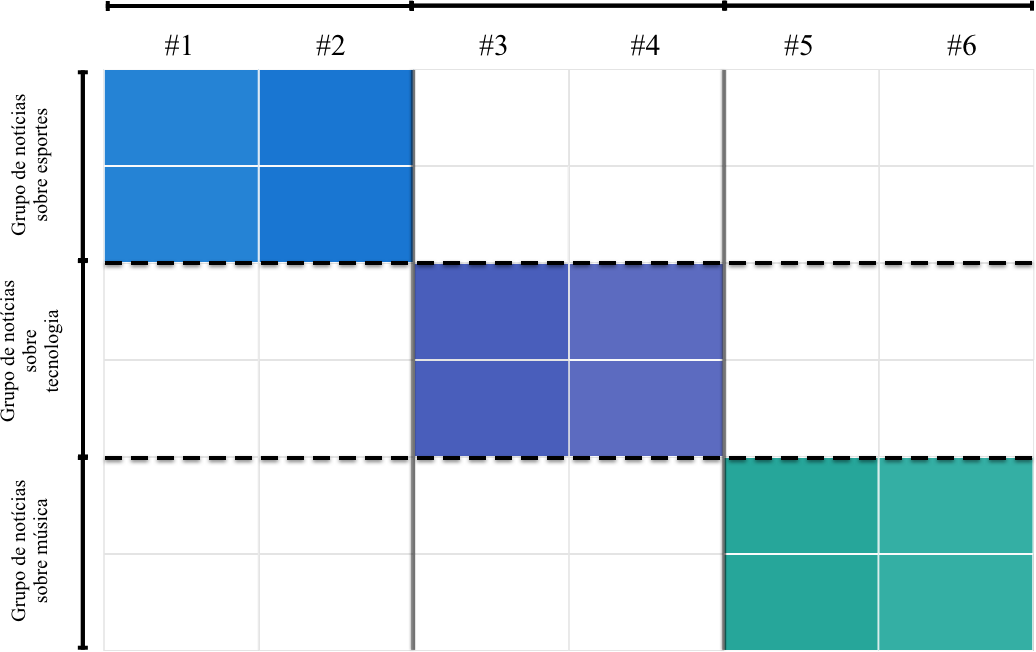
\includegraphics[scale=0.25]{img/sistema1-update.png}
  % \end{figure}
  \begin{itemize}
        \item Aplicação de mineração de textos
        \item Coleção de documentos $\rightarrow$ matriz de dados
        \item Contagem de palavras para cada documento
      \end{itemize}

  \begin{figure} [htpb]
    \centering
    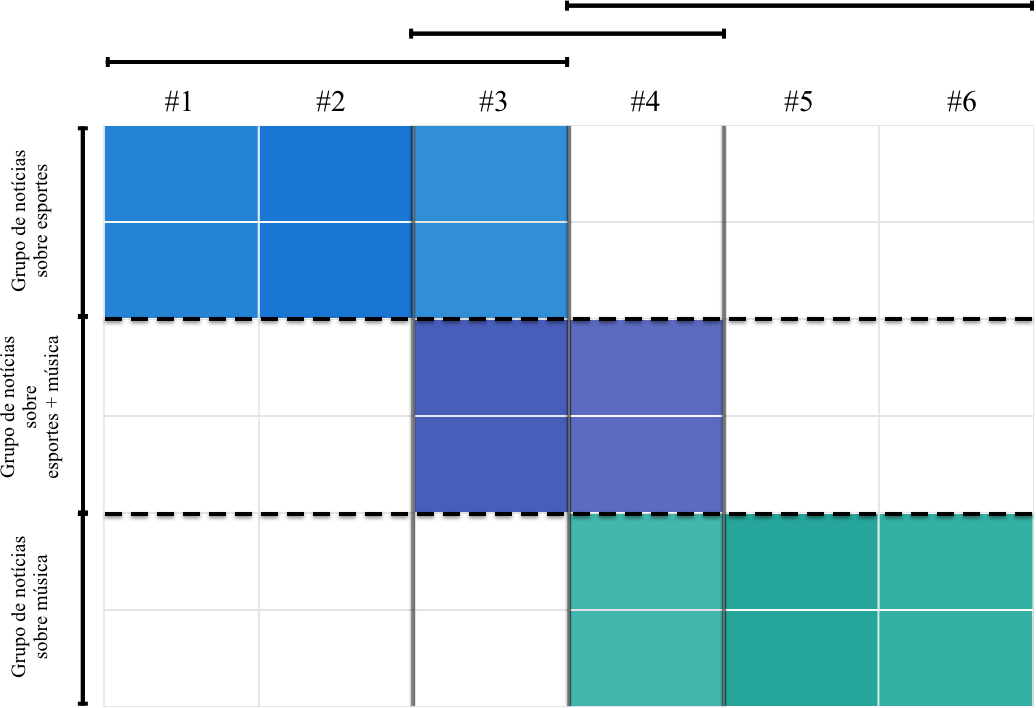
\includegraphics[scale=0.22]{img/sistema2.png}
  \end{figure}
\end{frame}

% %\subsection{Definição do problema}

% \begin{frame}
%   \frametitle{Coagrupamento}
%   \begin{itemize}
%     \item Matriz de dados: $X$ com $n$ linhas e $m$ colunas
%     \item Objetivo:
%     \begin{itemize}
%       \item Encontrar $k$ cogrupos de linhas:
%         $$\mathcal{K}_p, \forall p \in \{1, \dots, k\}$$
%       \item Encontrar $l$ cogrupos de colunas:
%         $$\mathcal{L}_q, \forall q \in \{1, \dots, l\}$$
%     \end{itemize}
%   \end{itemize}
% \end{frame}

%------------------------------------------------

% \begin{frame}
%   \frametitle{Fatoração de matrizes não-negativas}
%   \begin{itemize}
%     \item Matriz de dados: $X \in \mathbb{R}^{n \times m}$
%     \item Reconstrução: $X \approx USV^T$
%     \begin{itemize}
%       \item $U \in \mathbb{R}^{n \times k}$
%       \item $S \in \mathbb{R}^{k \times l}$
%       \item $V \in \mathbb{R}^{m \times l}$
%     \end{itemize}
%   \end{itemize}

% \end{frame}

%------------------------------------------------

\begin{frame}
  \frametitle{Problema e Hipótese}

  \begin{block}{Definição do problema}
    \begin{itemize}
      \item Definição do problema de coagrupamento com \textbf{sobreposição} de colunas em FM
      \item Soluções algorítmicas:
        \begin{itemize}
          \item Resolver coagrupamento
          \item \textbf{sobreposição} de cogrupos de colunas de forma adequada
        \end{itemize}
    \end{itemize}
  \end{block}

% \end{frame}

%------------------------------------------------

%\subsection{Hipótese}

% \begin{frame}
  % \frametitle{Hipótese}

  \begin{block}{Hipótese}
    \begin{itemize}
      \item \textbf{Sobreposição} de cogrupos de colunas pode ser resolvida por:
        $$X \approx g(U, S, V_{(1)}, \dots, V_{(k)})$$
      \item Permite que grupos de colunas sejam independentes
    \end{itemize}
  \end{block}

\end{frame}

%------------------------------------------------

%%\subsection{Objetivos}

\begin{frame}
\frametitle{Objetivos I}
  \begin{block}{Objetivo geral}
    \begin{itemize}
      \item Proposição do problema de coagrupamento com sobreposição de colunas
      \item Estratégias algorítmicas para resolver $X \approx g(U, S, V_{(1)}, \dots, V_{(k)})$:
    \begin{itemize}
      \item \textit{OvNMTF}
      \item \textit{BinOvNMTF}
    \end{itemize}
    \item Avaliando em termos de:
    \begin{itemize}
      \item capacidade de quantização e reconstrução
      \item capacidade de agrupamento
      \item capacidade de extração de informação (interpretabilidade)
    \end{itemize}
    \end{itemize}

  \end{block}
\end{frame}

%------------------------------------------------

\begin{frame}
  \frametitle{Objetivos II}

  \begin{block}{Objetivos específicos}
    \begin{itemize}
      \item Derivação formal para o \textit{OvNMTF} e \textit{BinOvNMTF}
      \item Aplicação do \textit{OvNMTF} e \textit{BinOvNMTF} em:
      \begin{itemize}
        \item ambientes controlados (bases de dados sintéticas)
        \item contexto de aplicação real (análise de dado textuais)
      \end{itemize}
      \item Novo conjunto de dados de notícias em língua portuguesa
    \end{itemize}

  \end{block}
\end{frame}

%------------------------------------------------

% \begin{frame}
%   \frametitle{Método}

%   \begin{itemize}
%     \item Análise exploratória da literatura sobre FM aplicado à coagrupamento
%     \item Estudo, implementação e análise dos algoritmos \textit{BVD}, \textit{ONMTF} e \textit{FNMTF}
%     \item Proposição dos algoritmos \textit{OvNMTF} e \textit{BinOvNMTF}
%     \item Análises utilizando bases de dados sintéticas e bases de dados textuais (iG e NIPS):
%     \begin{itemize}
%       \item inspeção visual e erro de quantização para análise da capacidade de reconstrução
%       \item técnicas de avaliação externa para análise da capacidade de agrupamento
%       \item análise empírica por meio de experimentos qualitativos para avaliação da capacidade de extração de informação e interpretabilidade dos modelos
%     \end{itemize}
%   \end{itemize}

% \end{frame}

%------------------------------------------------
\section{Conceitos Fundamentais}
%------------------------------------------------

%\subsection{Agrupamento}

\begin{frame}
  \frametitle{Definição de agrupamento}

  \begin{block}{Definição}
    \begin{itemize}
      \item Matriz de dados: $X \in \mathbb{R}^{n \times m}$
      \item Conjunto de vetores de linhas:
        $$\mathcal{N} = \{ \mathbf{x}_{1 \cdot}, \dots, \mathbf{x}_{n \cdot} \}$$
      \item Objetivo:
        \begin{itemize}
          \item Particionar $\mathcal{N}$:
           $$\mathcal{K}_p \subseteq \mathcal{N}, \forall p \in \{ 1, \dots, k\}$$
          \item Resultado:
            $$\mathscr{K} = \{\mathcal{K}_1, \dots, \mathcal{K}_k\}$$
        \end{itemize}
    \end{itemize}
  \end{block}

\end{frame}

%------------------------------------------------

% \begin{frame} [shrink=15]
%   \frametitle{Coagrupamento}

%   \begin{figure} [htpb]
%     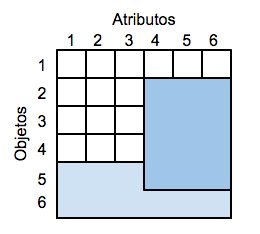
\includegraphics[width=0.8\textwidth]{img/bicluster.png}
%   \end{figure}
% \end{frame}

\begin{frame} [shrink=15]
  \frametitle{Definição de coagrupamento}
  \begin{block}{Definição}
    \begin{itemize}
      \item Matriz de dados: $X \in \mathbb{R}^{n \times m}$
      \item Conjunto de vetores de linhas:
        $$\mathcal{N} = \{ \mathbf{x}_{1 \cdot}, \dots, \mathbf{x}_{n \cdot} \}$$
      \item Conjunto de vetores de colunas
        $$\mathcal{M} = \{ \mathbf{x}_{\cdot 1}, \dots, \mathbf{x}_{\cdot m} \}$$
      \item Objetivo:
        \begin{itemize}
          \item Encontrar subconjuntos de $\mathcal{N}$:
            $$\mathcal{K}_p \subseteq \mathcal{N}, \forall p \in \{ 1, \dots, k\}$$
          \item Encontrar subconjuntos de $\mathcal{M}$:
            $$\mathcal{L}_q \subseteq \mathcal{M}, \forall q \in \{1, \dots, l\}$$
          \item Encontrar submatrizes de $X$:
            $$X_{\mathcal{K}_p \mathcal{L}_q}$$
        \end{itemize}
    \end{itemize}
  \end{block}
\end{frame}

% \begin{frame}
%   \frametitle{Cogrupos}
%   \begin{itemize}
%     \item Cogrupos diferem quanto aos seus tipos:
%     \begin{itemize}
%       \item com valores constantes, com valores constantes nas linhas ou colunas, com valores coerentes, com evoluções coerentes
%     \end{itemize}
%     \item ou quanto as suas estruturas
%   \end{itemize}

%   \begin{figure}[H]
%     \centering
%       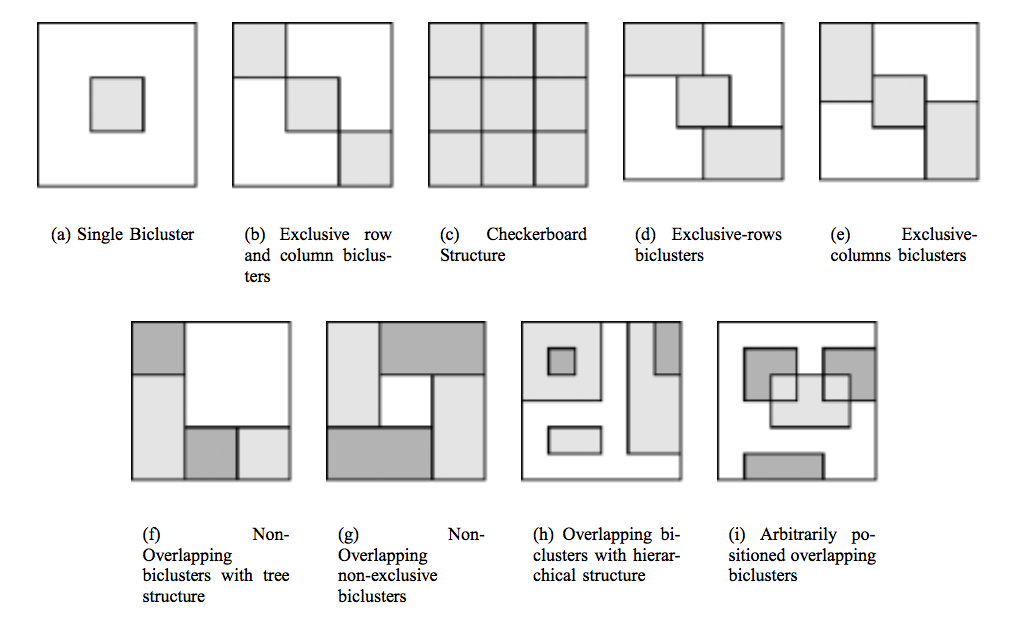
\includegraphics[width=0.7\textwidth]{img/synteticBiclusters.png}
%   \end{figure}

% \end{frame}

%------------------------------------------------

% \begin{frame}
% \frametitle{Fatoração de matrizes não-negativas para coagrupamento}
%   \begin{itemize}
%     \item NMF é um método capaz de extrair conhecimento através da análise das partes de um objeto
%     \item A ideia de análise por partes é usada para resolução da tarefa de coagrupamento
%     \item Aplicações:
%     \begin{itemize}
%       \item agrupamento de genes e análise de microarray em bioinformática
%       \item filtragem colaborativa em sistemas de recomendação
%       \item mineração de textos
%     \end{itemize}
%   \end{itemize}
% \end{frame}

%------------------------------------------------

\begin{frame}
\frametitle{Definição de coagrupamento em FM não-negativas}

  \begin{block}{Definição}
    \begin{itemize}
      \item Matriz de dados: $X \in \mathbb{R}^{n \times m}_{+}$
      \item Conjunto de vetores de linhas:
        $$\mathcal{N} = \{ \mathbf{x}_{1 \cdot}, \dots, \mathbf{x}_{n \cdot} \}$$
      \item Conjunto de vetores de colunas
        $$\mathcal{M} = \{ \mathbf{x}_{\cdot 1}, \dots, \mathbf{x}_{\cdot m} \}$$
      \item Objetivo:
        \begin{itemize}
          \item Particionar $\mathcal{N}$:
            $$\mathcal{K}_p \subseteq \mathcal{N}, \forall p \in \{ 1, \dots, k\}$$
          \item Particionar $\mathcal{M}$:
            $$\mathcal{L}_q \subseteq \mathcal{M}, \forall q \in \{1, \dots, l\}$$
          \item Resultado:
            $\mathscr{K} = \{\mathcal{K}_1, \dots, \mathcal{K}_k\}$
            $\mathscr{L} = \{\mathcal{L}_1, \dots, \mathcal{L}_l\}$
        \end{itemize}
    \end{itemize}
  \end{block}

\end{frame}

%------------------------------------------------

\section{Algoritmos de FM não-negativas para agrupamento e coagrupamento}

%------------------------------------------------

% \begin{frame}
%   \frametitle{K-means I}

%   \begin{block}{Problema \textit{k-means}}
%     \begin{equation}
%         \begin{array}{lclcl}
%             \displaystyle \mathcal{F}_1(U, C) & = & \displaystyle \min_{U, C} & \sum_{i=1}^n \sum_{p=1}^k u_{ip} \norm{\mathbf{x_{i \cdot} - \mathbf{c_{p \cdot}}}}^2 \\
%                                  &   & \text{suj. a} & U \in \Psi^{n \times k}, \\
%                                               &   & & C \in \mathbb{R}^{k \times m}, \\
%                                               &   & & \sum_{p=1}^{k} u_{ip} = 1, \forall i
%         \end{array} \nonumber
%     \end{equation}
%   \end{block}

% \end{frame}

%------------------------------------------------

\begin{frame}
  \frametitle{K-means}

  \begin{block}{Problema \textit{k-means} (forma fatoração)}
    \begin{equation}
        \begin{array}{lclcl}
            \displaystyle \mathcal{F}_1(U, C) & = & \displaystyle \min_{U, C} & \norm{X - UC}^{2}_{F} \\
                                              &   & \text{suj. a} & U \in \Psi^{n \times k}, \\
                                              &   & & C \in \mathbb{R}^{k \times m}, \\
                                              &   & & \sum_{p=1}^{k} u_{ip} = 1, \forall i
        \end{array} \nonumber
    \end{equation}
  \end{block}
\end{frame}

%------------------------------------------------

% \begin{frame}[shrink=15]
%   \frametitle{K-means}

%   \begin{algorithm}[H]
%       \begin{algorithmic}[1]
%           \Function{k-means}{$X$, $k$, $t_{max}$}
%               \State \textbf{Inicialize:} $C^{(0)} \gets \mathcal{U}(0, 1)$ e $t \gets 0$.
%               \While{(não convergiu) e ($t \leq t_{max}$)}
%                   \State
%                       \begin{equation}
%                           (U^{(t+1)})_{ip} \gets \left\{
%                               \begin{array}{ll}
%                                   1 & p = \argmin_{p' \in \{1, \dots, k\}} \norm{ \mathbf{x}_{i \cdot} - \mathbf{c}^{(t)}_{p' \cdot} }^2 \\
%                                   0 & \textit{caso contrário}
%                               \end{array}    \nonumber
%                           \right. \forall i, p
%                       \end{equation}
%                       \Comment{Etapa de Esperança}
%                   \State
%                       \begin{equation}
%                           (C^{(t+1)})_{p \cdot} \gets \frac{\sum_{i=1}^{n} u_{ip}^{(t+1)} \mathbf{x}_{i \cdot} }{\sum_{i=1}^{n} u_{ip}^{(t+1)}}, \forall p \text{ ou } C^{(t+1)} = (U^{(t+1)^T} U^{(t+1)})^{-1} U^{(t+1)^T} X \nonumber
%                       \end{equation}
%                       \Comment{Etapa de Maximização}
%                   \State $t \gets t + 1$
%               \EndWhile
%               \State \textbf{return} $U^{(t)}, C^{(t)}$
%           \EndFunction
%       \end{algorithmic}
%   \end{algorithm}

% \end{frame}

%------------------------------------------------

% \begin{frame}
%   \frametitle{Fuzzy K-means I}

%   \begin{block}{Problema \textit{fuzzy k-means}}
%     \begin{equation}
%         \begin{array}{lclcl}
%             \displaystyle \mathcal{F}_2(U, C) & = & \displaystyle \min_{U, C}    & \sum_{i=1}^n \sum_{p=1}^k u_{ip}^w \norm{\mathbf{x_{i \cdot} - \mathbf{c_{p \cdot}}}}^2 \\
%                                               &   & \text{suj. a}                & U \in \mathbb{R}^{n \times k}, \\
%                                               &   &                              & C \in \mathbb{R}^{k \times m}, \\
%                                               &   &                              & \sum_{p=1}^{k} u_{ip} = 1, \forall i
%         \end{array} \nonumber
%     \end{equation}
%     em que $w \in [1, 2, \dots, \infty]$.
%   \end{block}

% \end{frame}

%------------------------------------------------

\begin{frame}
  \frametitle{Fuzzy K-means}

  \begin{block}{Problema \textit{fuzzy k-means} ($w = 2$)}
    \begin{equation}
      \begin{array}{lclcl}
          \displaystyle \mathcal{F}^{w=2}_2(U, C) & = & \displaystyle \min_{U, C}    &  \norm{X - UC}^{2}_F \\
                                            &   & \text{suj. a}                & U \in \mathbb{R}^{n \times k}, \\
                                            &   &                              & C \in \mathbb{R}^{k \times m}, \\
                                            &   &                              & \sum_{p=1}^{k} u_{ip} = 1, \forall i
      \end{array} \nonumber
  \end{equation}
  \end{block}

\end{frame}

%------------------------------------------------

%\subsection{Coagrupamento}

% \begin{frame} [allowframebreaks]
%   \frametitle{Coagrupamento}

%   \begin{block}{Definição}
%     Uma das visões da tarefa de agrupamento é de encontrar submatrizes dentro de uma matriz de dados: tem-se uma matriz $X$, de dimensão $n \times m$, formada por um conjunto de vetores de linhas $\mathcal{N} = \{ \mathbf{x}_{1 \cdot}, \dots, \mathbf{x}_{n \cdot} \}$ e um conjunto de vetores de colunas $\mathcal{M} = \{ \mathbf{x}_{\cdot 1}, \dots, \mathbf{x}_{\cdot m} \}$.
%     \vspace{1em}
%     O problema de coagrupamento, dentro desta visão, é encontrar cogrupos, que são submatrizes de $X$, denotados por $X_{\mathcal{K}_p \mathcal{L}_q}$, considerando $k$ subconjuntos ordenados $\mathcal{K}_p \subseteq \mathcal{N}$, $l$ subconjuntos ordenados $\mathcal{L}_q \subseteq \mathcal{M}$, e os índices $p \in \{ 1, \dots, k\}$ e $q \in \{1, \dots, l\}$.
%     \vspace{1em}
%     Assim, o cogrupo $X_{\mathcal{K}_p \mathcal{L}_q}$ é um grupo dos dados em $\mathcal{K}_p$, perante as características em $\mathcal{L}_q$.
%   \end{block}

%   \begin{figure} [htpb]
%     \caption{Conjunto de dados com dois cogrupos}
%     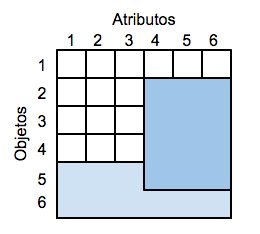
\includegraphics[width=0.55\textwidth]{img/bicluster.png}
%   \end{figure}

%   \begin{itemize}
%     \item Cogrupos diferem quanto aos seus tipos:
%     \begin{itemize}
%       \item com valores constantes, com valores constantes nas linhas ou colunas, com valores coerentes, com evoluções coerentes
%     \end{itemize}
%     \item ou quanto as suas estruturas
%   \end{itemize}

%   \begin{itemize}
%     \item Algoritmos: \textit{Cheng\&Church}, \textit{Spectral}, \textit{AiNet}
%     \item Avaliação: Internas, Externas
%   \end{itemize}

%   \begin{figure}[H]
%     \centering
%       \caption{Estruturas de cogrupos}
%       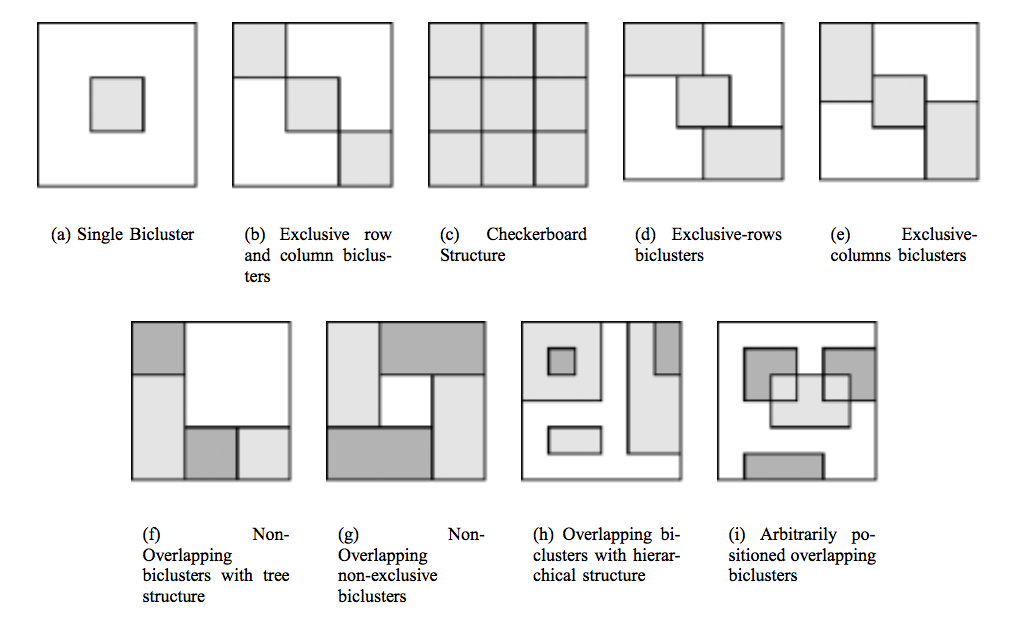
\includegraphics[width=0.7\textwidth]{img/synteticBiclusters.png}
%   \end{figure}

% \end{frame}

%------------------------------------------------

% \section{Fatoração de matrizes não-negativas para coagrupamento}

%------------------------------------------------

% \begin{frame}
% \frametitle{Fatoração de matrizes não-negativas para coagrupamento}
% \begin{itemize}
%   \item NMF é um método capaz de extrair conhecimento através da análise das partes de um objeto
%   \item A ideia de análise por partes é usada para resolução da tarefa de coagrupamento
%   \item Aplicações
%   \begin{itemize}
%     \item agrupamento de genes e análise de microarray em bioinformática
%     \item filtragem colaborativa em sistemas de recomendação
%     \item mineração de textos
%   \end{itemize}
% \end{itemize}
% \end{frame}

%------------------------------------------------

% \begin{frame}
% \frametitle{Fatoração de matrizes não-negativas para coagrupamento}

%   \begin{block}{Definição}
%     Algoritmos de coagrupamento baseados em NMF têm como entrada uma matriz de dados $X \in \mathbb{R}^{n \times m}_{+}$, contendo números reais positivos com $n$ linhas e $m$ colunas.

%     \vspace{0.5em}

%     Esta matriz é formada por um conjunto de vetores de linhas $\mathcal{N} = \{ \mathbf{x}_{1 \cdot}, \dots, \mathbf{x}_{n \cdot} \}$ e um conjunto de vetores de colunas $\mathcal{M} = \{ \mathbf{x}_{\cdot 1}, \dots, \mathbf{x}_{\cdot m} \}$, e as relações existentes entre cada linha $\mathbf{x}_{i \cdot}$ e cada coluna $\mathbf{x}_{\cdot j}$ são representadas por $x_{ij}$ considerando os índices $i \in \{1, \dots, n\}$ e $j \in \{1, \dots, m\}$, que é justamente um valor da matriz $X$.

%     \vspace{0.5em}

%     Cada valor em $x_{ij}$ representa, então, a relação existente entre pares de elementos em algum contexto de interesse.

%     \vspace{0.5em}

%     O objetivo é encontrar $k$ partições de $\mathcal{N}$, denotadas pelos subconjuntos ordenados $\mathcal{K}_p \subseteq \mathcal{N}$, $l$ partições para $\mathcal{M}$, denotadas pelos subconjuntos ordenados $\mathcal{L}_q \subseteq \mathcal{M}$, considerando os índices $p \in \{ 1, \dots, k\}$ e $q \in \{1, \dots, l\}$.

%     \vspace{0.5em}

%     Então, os conjuntos $\{\mathcal{K}_1, \dots, \mathcal{K}_k\}$ e $\{\mathcal{L}_1, \dots, \mathcal{L}_l\}$ são os cogrupos de linhas e colunas, respectivamente.
%   \end{block}

% \end{frame}

%------------------------------------------------

%\subsection{Decomposição de valores em blocos para coagrupamento}

% \begin{frame} [allowframebreaks]
%   \frametitle{Decomposição de valores em blocos para coagrupamento}

%   \begin{figure}[H]
%     \centering
%     \caption{Fatoração da matriz original de dados $X$ em três outras matrizes: $U$, $S$ e $V$}
%     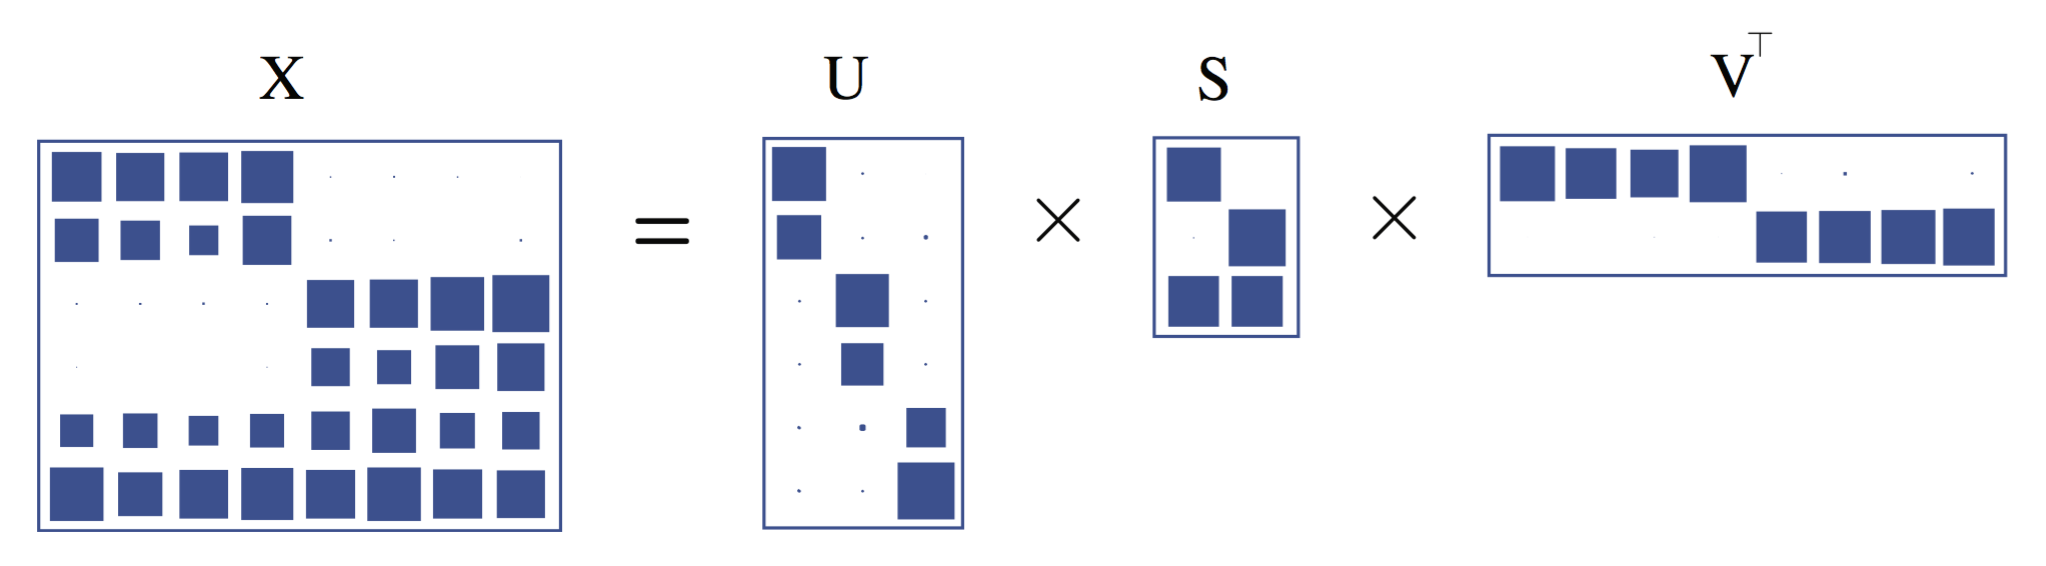
\includegraphics[width=0.8\textwidth]{img/factorizationXUSV.png}
%   \end{figure}

%   \begin{figure}[H]
%     \centering
%     \caption{A reconstrução da primeira linha $\mathbf{x}_{1 \cdot}$ de $X$, através da multiplicação da matriz indicadora de grupos de linhas $U$ pela matriz dos protótipos de linhas $(S V^T)$.}
%     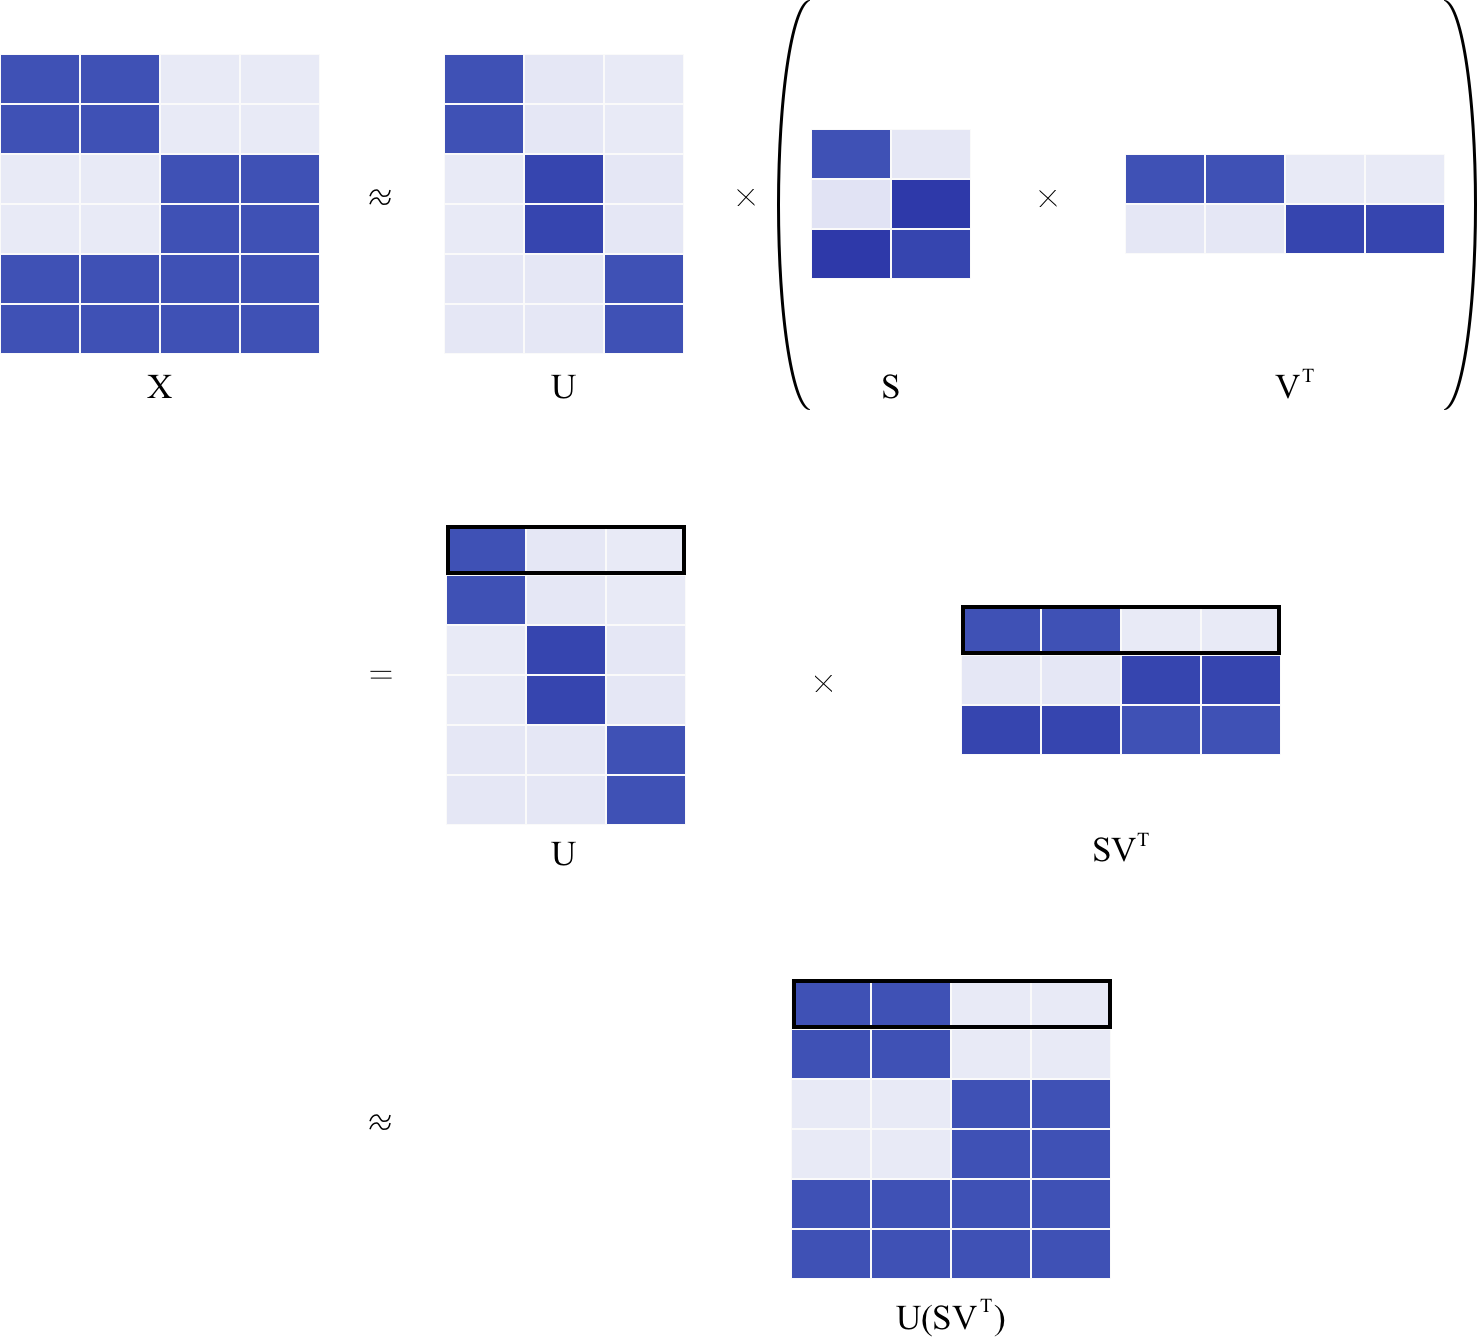
\includegraphics[width=0.6\textwidth]{img/reconstruction.png}
%   \end{figure}

\begin{frame}
  \frametitle{FM não-negativas para coagrupamento (BVD)}
  \begin{block}{Problema \textit{BVD}}
    \begin{equation}
        \begin{array}{lclcl}
            \displaystyle \mathcal{F}_3(U, S, V) & = & \displaystyle \min_{U, S, V} & \norm{X - USV^T}^{2}_{F} \\
                                               &   & \text{suj. a}                & U \geq 0, S \geq 0, V \geq 0
        \end{array}   \nonumber
    \end{equation}
  \end{block}

\end{frame}

%------------------------------------------------

% \begin{frame}[shrink=15]
%   \frametitle{Algoritmo para Decomposição de valores em blocos para coagrupamento}

%   \begin{algorithm}[H]
%   % \caption{Algoritmo baseado em atualização multiplicativa para solução do \textit{BVD}}
%   \begin{algorithmic}[1]
%   \Function{BVD}{$X$, $k$, $l$, $t_{max}$}
%   \State \textbf{Inicialize:} $U^{(0)} \gets \mathcal{U}(0, 1), V^{(0)} \gets \mathcal{U}(0, 1), S^{(0)} \gets \frac{1}{nm} \sum_{i, j} x_{ij}$ e $t \gets 0$.
%   \While{(não convergiu) e ($t \leq t_{max}$)} %\Comment{We have the answer if r is 0}
%   \State
%   \begin{equation}
%   \label{eq:bvd:updateU}
%   U^{(t+1)} \gets U^{(t)} \odot \frac{ X V^{(t)} S^{(t)^T} }{ U^{(t)} S^{(t)} V^{(t)^T} V^{(t)} S^{(t)^T }}             \nonumber
%   \end{equation}
%   \State
%   \begin{equation}
%   \label{eq:bvd:updateV}
%   V^{(t+1)} \gets V^{(t)} \odot \frac{ X^T U^{(t+1)} S^{(t)} }{ V^{(t)} S^{(t)^T} U^{(t+1)^T} U^{(t+1)} S^{(t)} }       \nonumber
%   \end{equation}
%   \State
%   \begin{equation}
%   \label{eq:bvd:updateS}
%   S^{(t+1)} \gets S^{(t)} \odot \frac{ U^{(t+1)^T} X V^{(t+1)} }{ U^{(t+1)^T} U^{(t+1)} S^{(t)} V^{(t+1)^T} V^{(t+1)} } \nonumber
%   \end{equation}
%   \State $t \gets t + 1$
%   \EndWhile\label{euclidendwhile}
%   \State \textbf{return} $U^{(t)}, S^{(t)}, V^{(t)}$
%   \EndFunction
%   \end{algorithmic}
%   \end{algorithm}

% \end{frame}

%------------------------------------------------

% \begin{frame}
%   \frametitle{Pós-processamento para Decomposição de valores em blocos para coagrupamento}

%   Note que como $U$ e $V$ possuem valores no domínio dos reais, então, não é possível obter as partições diretamente, sem um processo de pós-processamento.
%   Um modo simples de obter o particionamento para as linhas toma a seguinte forma:
%   $$\mathcal{K}_{p}=\{\mathbf{x}_{i\cdot}~|~i\in\{1,\dots,n\}\text{ e }p=\argmax_{p'\in\{1,\dots,k\}} u_{ip'} \}, \forall p\in\{1,\dots,k\}$$

% \end{frame}

%------------------------------------------------

%\subsection{Fatoração ortogonal tripla de matrizes não-negativas}

\begin{frame}
  \frametitle{FM não-negativas ortogonal tripla (ONMTF)}

  % \begin{figure} [htpb]
  % \centering
  % \caption{Base de protótipos obtidas com NMF sem restrições (a) e com restrições de ortogonalidade nas matrizes}
  % \begin{subfigure}[b]{0.3\textwidth}
  % 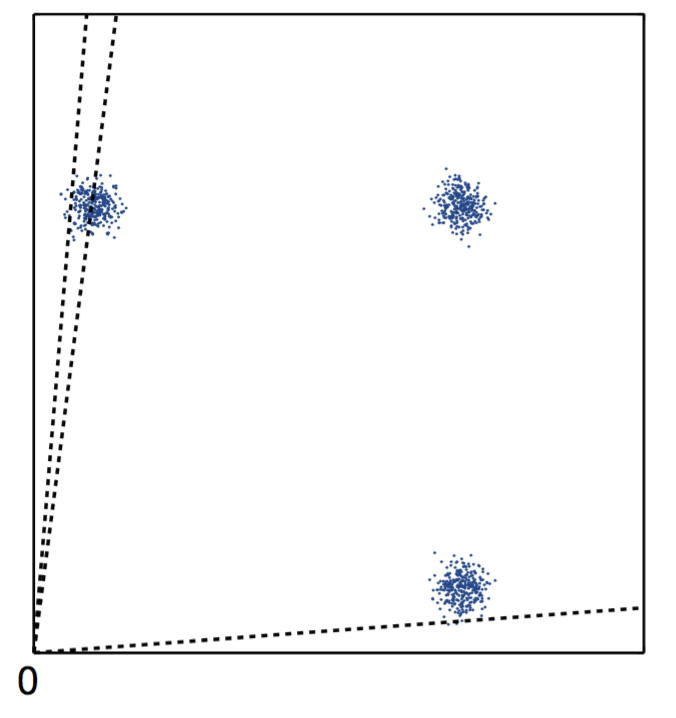
\includegraphics[width=\textwidth]{img/bvdVsOnmtf1.png}
  % \caption{}
  % \label{fig:bvdvsonmtf:1}
  % \end{subfigure}
  % ~ %add desired spacing between images, e. g. ~, \quad, \qquad, \hfill etc.
  % %(or a blank line to force the subfigure onto a new line)
  % \begin{subfigure}[b]{0.3\textwidth}
  % 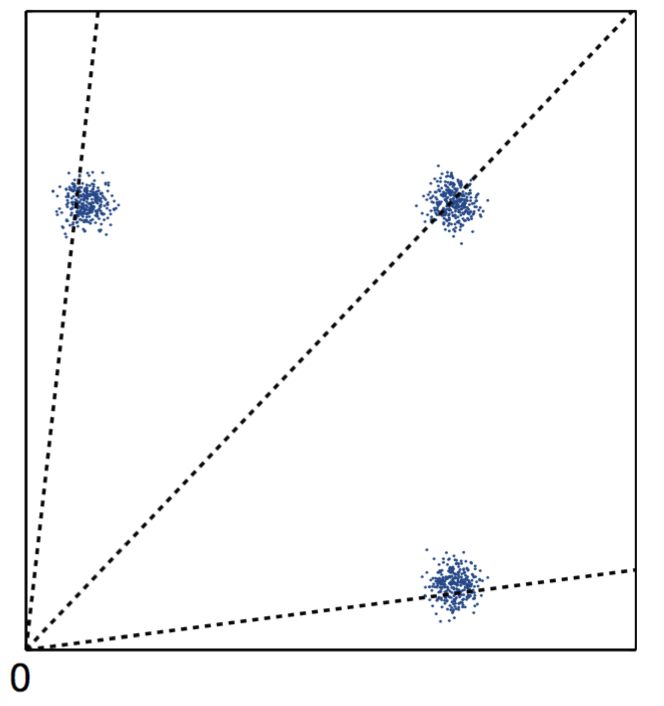
\includegraphics[width=\textwidth]{img/bvdVsOnmtf2.png}
  % \caption{}
  % \label{fig:bvdvsonmtf:2}
  % \end{subfigure}
  % \end{figure}

  \begin{block}{Problema \textit{ONMTF}}
    \begin{equation}
        \begin{array}{lclcl}
            \displaystyle \mathcal{F}_6(U, S, V) & = & \displaystyle \min_{U, S, V} & \norm{X - USV^T}^{2}_{F}      \\
                                                 &   & \text{suj. a}                & U \geq 0, S \geq 0, V \geq 0, \\
                                                 &   &                              & U^T U = I,                    \\
                                                 &   &                              & V^T V = I
        \end{array}   \nonumber
    \end{equation}
  \end{block}

\end{frame}

%------------------------------------------------

% \begin{frame}[shrink=15]
%   \frametitle{Algoritmo para Fatoração ortogonal tripla de matrizes não-negativas}

%   \begin{algorithm}[H]
%   \label{algo:onmtf}
%   \begin{algorithmic}[1]
%   \Function{ONM3F}{$X$, $k$, $l$, $t_{max}$}
%   \State \textbf{Inicialize:} $U^{(0)} \gets \mathcal{U}(0, 1), V^{(0)} \gets \mathcal{U}(0, 1), S^{(0)} \gets \mathcal{U}(0, 1)$ e $t \gets 0$.
%   \While{(não convergiu) e ($t \leq t_{max}$)} %\Comment{We have the answer if r is 0}
%   \State
%   \begin{equation}
%   \label{eq:onmtf:updateU}
%   U^{(t+1)} \gets U^{(t)} \odot \sqrt{ \frac{ X V^{(t)} S^{(t)^T} }{ U^{(t)} U^{(t)^T} X V^{(t)} S^{(t)^T} } }
%   \end{equation}
%   \State
%   \begin{equation}
%   \label{eq:onmtf:updateV}
%   V^{(t+1)} \gets V^{(t)} \odot \sqrt{ \frac{ X^T U^{(t+1)} S }{ V^{(t)} V^{(t)^T} X^T U^{(t+1)} S^{(t)} } }
%   \end{equation}
%   \State
%   \begin{equation}
%   \label{eq:onmtf:updateS}
%   S^{(t+1)} \gets S^{(t)} \odot \sqrt{ \frac{ U^{(t+1)^T} X V^{(t+1)} }{ U^{(t+1)^T} U^{(t+1)} S^{(t)} V^{(t+1)^T} V^{(t+1)} } }
%   \end{equation}
%   \State $t \gets t + 1$
%   \EndWhile\label{euclidendwhile}
%   \State \textbf{return} $U^{(t)}, S^{(t)}, V^{(t)}$
%   \EndFunction
%   \end{algorithmic}
%   \end{algorithm}

% \end{frame}

%------------------------------------------------

% \begin{frame}
%   \frametitle{Algoritmo para Fatoração ortogonal tripla de matrizes não-negativas}

%   \begin{itemize}
%     \item Uma outra derivação simplificada para o problema do ONMTF
%     \item Considere uma função de otimização qualquer $\mathcal{J}$ e seu respectivo gradiente $\nabla \mathcal{J}$:
%     \[
%       \begin{array}{lclcl}
%       \nabla \mathcal{J} & = & [\nabla \mathcal{J}]^+ - [\nabla \mathcal{J}]^-
%       \end{array}
%     \]
%     \item Se $[\nabla \mathcal{J}]^+ \geq 0$ e $[\nabla \mathcal{J}]^- \geq 0$, então, é possível definir uma regra de atualização multiplicativa, para otimizar os parâmetros $\Theta$ da função $\mathcal{J}$:

%       \begin{equation}
%       \label{eq:onmtf:updateTheta}
%       \Theta \gets \Theta \odot \left ( \frac{ [\nabla \mathcal{J}]^- }{ [\nabla \mathcal{J}]^+ } \right )^{\cdot \eta} \nonumber
%       \end{equation}

%       onde $(\cdot)^{\cdot \eta}$ representa a potência para cada elemento, e $\eta$ uma taxa de aprendizado ($0 < \eta \leq 1$).
%   \end{itemize}

% \end{frame}

%------------------------------------------------

% \begin{frame}[shrink=15]
%   \frametitle{Algoritmo baseado na superfície com restrições para Fatoração ortogonal tripla de matrizes não-negativas}

%   \begin{algorithm}[H]
%   \label{algo:onmtf2}
%   \begin{algorithmic}[1]
%   \Function{ONMTF}{$X$, $k$, $l$, $t_{max}$}
%   \State \textbf{Inicialize:} $U^{(0)} \gets \mathcal{U}(0, 1), V^{(0)} \gets \mathcal{U}(0, 1), S^{(0)} \gets \mathcal{U}(0, 1)$ e $t \gets 0$.
%   \While{(não convergiu) e ($t \leq t_{max}$)} %\Comment{We have the answer if r is 0}
%   \State
%   \begin{equation}
%   U^{(t+1)} \gets U^{(t)} \odot \frac{ X V^{(t)} S^{(t)^T} }{ U^{(t)} S^{(t)} V^{(t)^T} X^T U^{(t)} } \nonumber
%   \end{equation}
%   \State
%   \begin{equation}
%   V^{(t+1)} \gets V^{(t)} \odot \frac{ X^T U^{(t+1)} S^{(t)} }{ V^{(t)} S^{(t)^T} U^{(t+1)^T} X V^{(t)} } \nonumber
%   \end{equation}
%   \State
%   \begin{equation}
%   S^{(t+1)} \gets S^{(t)} \odot \frac{ U^{(t+1)^T} X V^{(t+1)} }{ U^{(t+1)^T} U^{(t+1)} S^{(t)} V^{(t+1)^T} V^{(t+1)} } \nonumber
%   \end{equation}
%   \State $t \gets t + 1$
%   \EndWhile\label{euclidendwhile}
%   \State
%   $$U^{(t)} \gets U^{(t)} \diag(S^{(t)} \diag(\mathbf{1}^T V^{(t)}) \mathbf{1})$$
%   \State
%   $$V^{(t)} \gets V^{(t)} \diag(\mathbf{1}^T \diag(\mathbf{1}^T U^{(t)}) S^{(t)})$$
%   \State \textbf{return} $U^{(t)}, S^{(t)}, V^{(t)}$
%   \EndFunction
%   \end{algorithmic}
%   \end{algorithm}

% \end{frame}

%------------------------------------------------

%\subsection{Fatoração Tripla Rápida de Matrizes Não-negativas}

\begin{frame}
  \frametitle{Fatoração tripla rápida de matrizes não-negativas (FNMTF)}

  \begin{block}{Problema \textit{FNMTF}}
    \begin{equation}
        \begin{array}{lclcl}
            \displaystyle \mathcal{F}_7(U, S, V) & = & \displaystyle \min_{U, S, V} & \norm{X - USV^T}^{2}_{F} \\
                                                 &   & \text{suj. a}                & U \in \Psi^{n \times k}, \\
                                                 &   &                              & V \in \Psi^{m \times l}, \\
                                                 &   &                              & \sum_{p=1}^{k} u_{ip} = 1, \forall i, \\
                                                 &   &                              & \sum_{q=1}^{l} v_{jq} = 1, \forall j
        \end{array} \nonumber
    \end{equation}
  \end{block}

\end{frame}

%------------------------------------------------

% \begin{frame}[shrink=15]
%   \frametitle{Algoritmo para Fatoração Tripla Rápida de Matrizes Não-negativas}

%   \begin{algorithm}[H]
%   \label{algo:fnmtf}
%   \begin{algorithmic}[1]
%   \Function{FNMTF}{$X$, $k$, $l$, $t_{max}$}
%   \State \textbf{Inicialize:} $U^{(0)}, V^{(0)} \gets {0,1}~|~\sum_{p=1}^{k} u_{ip} = 1, \sum_{q=1}^{l} v_{jq} = 1, \forall i, j$, $S^{(0)} \gets \mathcal{U}(0, 1)$ e $t \gets 0$.
%   \While{(não convergiu) e ($t \leq t_{max}$)}
%   \State
%   \begin{equation}
%   \label{eq:fnmtf:updateS}
%   S^{(t+1)} \gets (U^{(t)^T} U^{(t)})^{-1} U^{(t)^T} X V^{(t)} (V^{(t)^T} V^{(t)})^{-1}   \nonumber
%   \end{equation}
%   \State
%   \[
%   \widetilde{V} \gets S^{(t+1)} V^{(t)^T}
%   \]
%   \State
%   \begin{equation}
%   \label{eq:fnmtf:updateF}
%   (U^{(t+1)})_{ip} \gets \left\{
%   \begin{array}{ll}
%   1 & p = \argmin_{p' \in \{1, \dots, k\}} \norm{ \mathbf{x}_{i \cdot} - \widetilde{\mathbf{v}}_{p' \cdot} }^2 \\
%   0 & \textit{caso contrário}
%   \end{array}    \nonumber
%   \right. \forall i, p
%   \end{equation}
%   \State
%   \[
%   \widetilde{U} \gets U^{(t+1)} S^{(t+1)}
%   \]
%   \State
%   \begin{equation}
%   \label{eq:fnmtf:updateG}
%   (V^{(t+1)})_{jq} \gets \left\{
%   \begin{array}{ll}
%   1 & q = \argmin_{q' \in \{1, \dots, l\}} \norm{ \mathbf{x}_{\cdot j} - \widetilde{\mathbf{u}}_{\cdot q'} }^2 \\
%   0 & \textit{caso contrário}
%   \end{array}      \nonumber
%   \right. \forall j, q
%   \end{equation}
%   \State $t \gets t + 1$
%   \EndWhile\label{euclidendwhile}
%   \State \textbf{return} $U^{(t)}, S^{(t)}, V^{(t)}$
%   \EndFunction
%   \end{algorithmic}
%   \end{algorithm}

% \end{frame}

\begin{frame}
\frametitle{Resumo das fatorações da literatura}

  \begin{table}[H]
  \centering
    \resizebox{\linewidth}{!}{\begin{tabular}{lccc}
        \hline
        & \textbf{Fatoração} & \textbf{Compactação} & \textbf{Restrições} \\
        \hline
        \textit{k-means}        & $X \approx UC$ & $n + km$ & $U \in \Psi^{n \times k}, C \in \mathbb{R}^{k \times m}, \sum_{p=1}^{k} u_{ip} = 1$ \\
        \hline \\
        \textit{fuzzy k-means}        & $X \approx UC$ & $nk + km$ & $U \in \mathbb{R}^{n \times k}, C \in \mathbb{R}^{k \times m}, \sum_{p=1}^{k} u_{ip} = 1$ \\
        \hline \\
        \textit{BVD}        & $X \approx USV^T$ & $nk + kl + ml$ & $U \geq 0, S \geq 0, V \geq 0$ \\
        \hline \\
        \textit{ONMTF}        & $X \approx USV^T$ & $nk + kl + ml$ & $U \geq 0, S \geq 0, V \geq 0, U^TU = I, V^TV = I$ \\
        \hline \\
        \textit{FNMTF}        & $X \approx USV^T$ & $n + kl + m$ & $U \in \Psi^{n \times k}, V \in \Psi^{m \times l}, \sum_{p=1}^{k} u_{ip} = 1, \sum_{q=1}^{l} v_{jq} = 1$ \\
        \hline \\
    \end{tabular}
    }
  \end{table}

\end{frame}

%------------------------------------------------

\section{Fatoração de matrizes não-negativas para coagrupamento com sobreposição de colunas}

%------------------------------------------------

% \begin{frame}
% \frametitle{Exemplo de aplicação para fatoração de matrizes não-negativas para coagrupamento com sobreposição de colunas}

%   \begin{figure}[H]
%   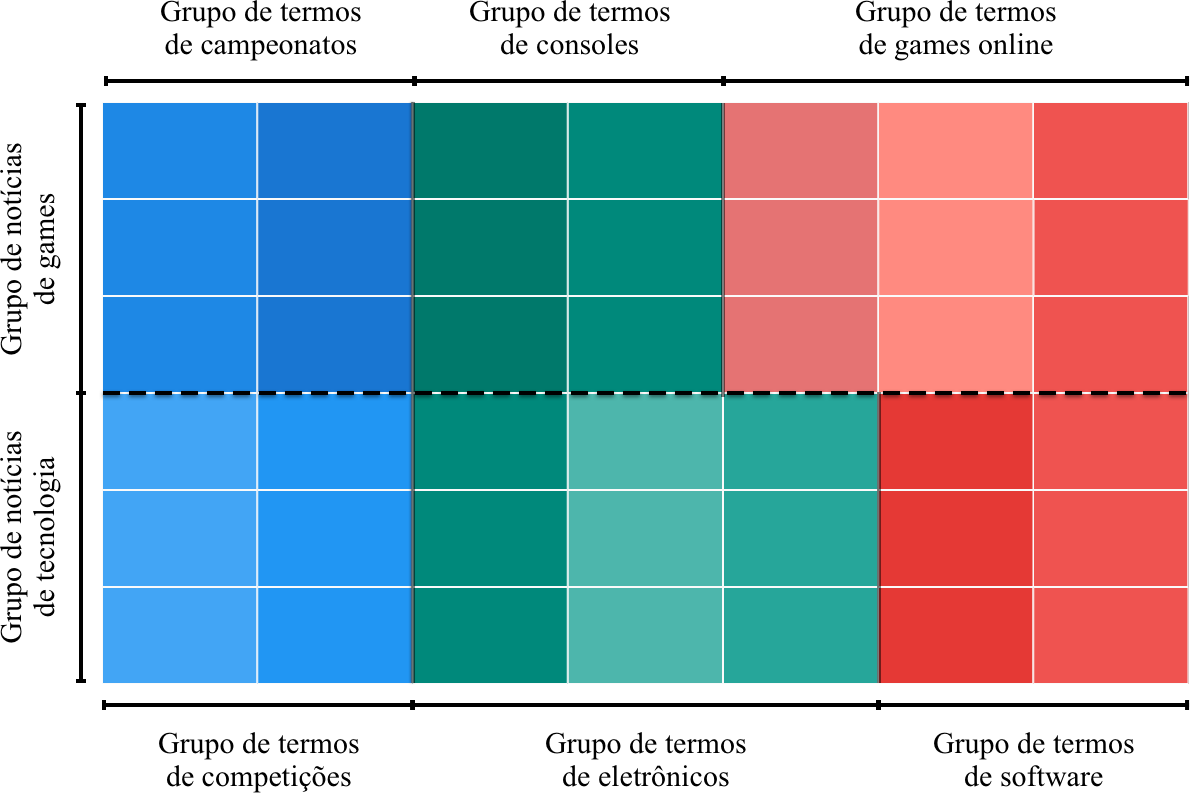
\includegraphics[width=0.8\textwidth]{img/ovnmtfNewsApplication.png}
%   \end{figure}

% \end{frame}

\begin{frame}
\frametitle{Fatoração de matrizes não-negativas para coagrupamento com sobreposição de colunas}

  \begin{figure}[H]
  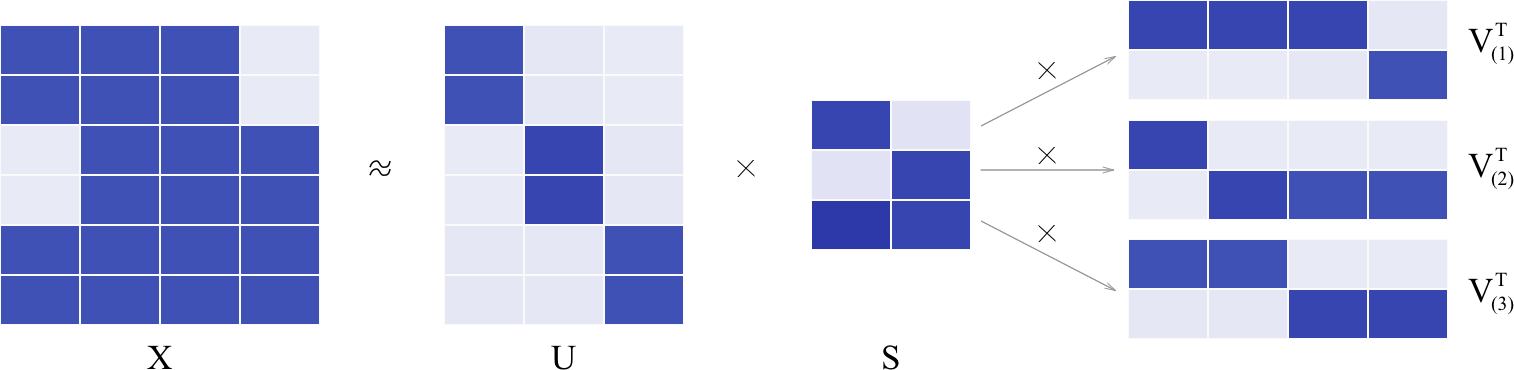
\includegraphics[width=1.0\textwidth]{img/factorizationXUSV1tok.png}
  \end{figure}

  \begin{itemize}
    \item $k$ particionamentos para as colunas ($V_{p}$)
    \item independência
  \end{itemize}

\end{frame}

\begin{frame} %[shrink=15]
\frametitle{Definição de fatoração de matrizes não-negativas para coagrupamento com sobreposição de colunas}

  \begin{block}{Definição}
    \begin{itemize}
      \item Matriz de dados: $X \in \mathbb{R}^{n \times m}_{+}$
      \item Conjunto de vetores de linhas:
        $\mathcal{N} = \{ \mathbf{x}_{1 \cdot}, \dots, \mathbf{x}_{n \cdot} \}$
      \item Conjunto de vetores de colunas:
        $\mathcal{M} = \{ \mathbf{x}_{\cdot 1}, \dots, \mathbf{x}_{\cdot m} \}$
    \end{itemize}
  \end{block}

  \begin{itemize}
  \item Objetivo:
        \begin{itemize}
          \item Particionar $\mathcal{N}$:
            $$\mathcal{K}_p \subseteq \mathcal{N}, \forall p \in \{ 1, \dots, k\}$$
          \item Particionar $\mathcal{M}$ $k$ vezes:
            $$\mathcal{L}_{pq} \subseteq \mathcal{M}, \forall p \in \{ 1, \dots, k\}, \forall q \in \{1, \dots, l\}$$
          \item Resultado:
            $$\mathscr{K} = \{\mathcal{K}_1, \dots, \mathcal{K}_k\}$$
            $$\mathscr{L} = \{\mathcal{L}_{11}, \dots, \mathcal{L}_{1l}, \dots, \mathcal{L}_{k1}, \dots \mathcal{L}_{kl}\}$$
        \end{itemize}
    \end{itemize}

\end{frame}

%------------------------------------------------

%\subsection{Fatoração Tripla de Matrizes Não-negativas com Sobreposição}

\begin{frame}
  \frametitle{Fatoração Tripla de Matrizes Não-negativas com Sobreposição (OvNMTF)}

  \begin{block}{Problema \textit{OvNMTF}}
    \begin{equation}
        \begin{array}{lclc}
            \displaystyle \mathcal{F}_6(U, S, V_{(1)}, \dots, V_{(k)}) & = & \displaystyle \min_{U, S, V_{(1)}, \dots, V_{(k)}} & \norm{X - U\sum_{p=1}^{k}I_{(p)}SV_{(p)}^T}^{2}_{F} \\
                                                                       &   & \text{suj. a}                & U \geq 0, S \geq 0, \\
                                                                       &   &                              & V_{(p)} \geq 0, \quad \forall p
        \end{array} \nonumber
    \end{equation}
    \begin{itemize}
      \item $I_{(p)} \in \{0,1\}^{k \times k}$ matriz seletora
    \end{itemize}
  \end{block}

\end{frame}

%------------------------------------------------

% \begin{frame}[shrink=15]
%   \frametitle{Algoritmo para Fatoração Tripla de Matrizes Não-negativas com Sobreposição}

%   \begin{algorithm}[H]
%   \label{algo:ovnmtf}
%       \begin{algorithmic}[1]
%           \Function{OvNMTF}{$X$, $k$, $l$, $t_{max}$}
%               \State \textbf{Inicialize:} $U^{(0)} \gets \mathcal{U}(0,1), S^{(0)} \gets \mathcal{U}(0,1), V_{(p)}^{(0)} \gets \mathcal{U}(0,1), \forall p$ e $t \gets 0$.
%               \While{(não convergiu) e ($t \leq t_{max}$)} %\Comment{We have the answer if r is 0}
%                   \State
%                       \begin{equation}
%                       \label{eq:ovnmtf:updateU}
%                           U^{(t+1)} \gets U^{(t)} \odot \frac{ \sum_{p=1}^{k} X V^{(t)}_{(p)} S^{(t)^T} I_{(p)} }{ \sum_{p=1}^{k} \sum_{p'=1}^k U^{(t)} I_{(p)} S^{(t)} V^{(t)^T}_{(p)} V^{(t)}_{(p')} S^{(t)^T} I_{(p')} }
%                       \end{equation}
%                   \For{$p \leftarrow 1 \text{ até } k$}
%                       \State
%                           \begin{equation}
%                           \label{eq:ovnmtf:updateV}
%                               V^{(t+1)}_{(p)} \gets V^{(t)}_{(p)} \odot \frac{ X^T U^{(t+1)} I_{(p)} S^{(t)} }{ \sum_{p'=1}^{k} V_{(p')} S^T I_{(p')} U^T U I_{(p)} S }
%                           \end{equation}
%                   \EndFor
%                   \State
%                       \begin{equation}
%                       \label{eq:ovnmtf:updateS}
%                           S^{(t+1)} \gets S^{(t)} \odot \frac{ \sum_{p=1}^{k} I_{(p)} U^{(t+1)^T} X V^{(t+1)}_{(p)} }{ \sum_{p=1}^{k} \sum_{p'=1}^{k} I_{(p)} U^{(t+1)^T} U^{(t+1)} I_{(p')} S^{(t)} V^{(t+1)^T}_{(p')} V^{(t+1)}_{(p)} }
%                       \end{equation}
%                   \State $t \gets t + 1$
%               \EndWhile\label{euclidendwhile}
%               \State \textbf{return} $U^{(t)}, S^{(t)}, V_{(1)}^{(t)}, \dots, V_{(k)}^{(t)}$
%           \EndFunction
%       \end{algorithmic}
%   \end{algorithm}

% \end{frame}

%------------------------------------------------

% \begin{frame}
%   \frametitle{Pós-processamento para Fatoração Tripla de Matrizes Não-negativas com Sobreposição}

%   O particionamento, neste caso, não é direto, então é necessário um processo de pós-processamento para a matriz $U$ e para as matrizes $V_{(1)}, \dots, V_{(k)}$.
%   Um modo simples de obter o particionamento para as linhas, é o seguinte:
%   \[
%       \mathcal{K}_{p}=\{x_{i\cdot}~|~i\in\{1,\dots,n\}\text{ e }p=\argmax_{p'\in\{1,\dots,k\}} u_{ip'} \}, \forall p\in\{1,\dots,k\}
%   \]

%   Pode-se usar a mesma estratégia para o particionamento das colunas:
%   \begin{align*}
%       \mathcal{L}_{pq} = \{ \mathbf{x}_{\cdot j}~|~j \in \{1, \dots, m \} \text{ e } q = \argmax_{q' \in \{1, \dots, l\}} v_{(p)_{j q'}} \}, \\
%       \forall j \in \{1, \dots, m\}, \forall q, q' \in \{1, \dots, l\}, \forall p \in \{1, \dots, k\}
%   \end{align*}

% \end{frame}

%------------------------------------------------

%\subsection{Fatoração Binária Tripla de Matrizes Não-negativas com Sobreposição}

\begin{frame}
  \frametitle{Fatoração Binária Tripla de Matrizes Não-negativas com Sobreposição (BinOvNMTF)}

  \begin{block}{Problema \textit{BinOvNMTF}}
    \begin{equation}
        \begin{array}{lclc}
            \displaystyle \mathcal{F}_7(U, S, V_{(1)}, \dots, V_{(k)}) & = & \displaystyle \min_{U, S, V_{(1)}, \dots, V_{(k)}} & \norm{ X - U \sum_{p=1}^{k} I_{(p)} S V_{(p)}^T }^{2}_{F} \\
                                                                       &   & \text{suj. a}                & U \in \Psi^{n \times k}, \\
                                                                       &   &                              & V_{(p)} \in \Psi^{m \times l}, \quad \forall p, \\
                                                                       &   &                              & \sum_{p=1}^{k} u_{ip} = 1, \forall i, \\
                                                                       &   &                              & \sum_{q=1}^{l} v_{(p)_{jq}} = 1, \forall p, j
        \end{array}   \nonumber
    \end{equation}
  \end{block}

\end{frame}

%------------------------------------------------

% \begin{frame}[shrink=15]
%   \frametitle{Algoritmo para Fatoração Binária Tripla de Matrizes Não-negativas com Sobreposição}

%   \begin{algorithm}[H]
%   \label{algo:binovbnmtf}
%       \begin{algorithmic}[1]
%           \Function{BinOvNMTF}{$X$, $k$, $l$, $t_{max}$}
%               \State \textbf{Inicialize:} $U^{(0)} \gets 0, 1 ~|~ \sum_{p=1}^{k} u_{ip} = 1$, $V_{(p)}^{(0)} \gets 0, 1 ~|~ \sum_{q=1}^{l} v_{(p)_{jq}} = 1, \forall i, j, p$ e $t \gets 0$.
%               \While{(não convergiu) e ($t \leq t_{max}$)}
%                   \State
%                       \begin{equation}
%                       \label{eq:binovbnmtf:updateS}
%                           S^{(t+1)} \gets \sum_{p=1}^k I_{(p)} (U^{(t)^T} U^{(t)})^{-1} U^{(t)^T} X V_{(p)}^{(t)} (V_{(p)}^{(t)^T} V_{(p)}^{(t)})^{-1}
%                       \end{equation}
%                   \State
%                       \[
%                           \widetilde{V} \gets \sum_{p=1}^k I_{(p)} S^{(t+1)} V_{(p)}^{(t)^T}
%                       \]
%                   \State
%                       \begin{equation}
%                       \label{eq:binovbnmtf:updateF}
%                           (U^{(t+1)})_{ip} \gets \left\{
%                               \begin{array}{ll}
%                                   1 & p = \argmin_{p' \in \{1, \dots, k\}} \norm{ \mathbf{x}_{i \cdot} - \mathbf{\widetilde{v}}_{p' \cdot} }^2 \\
%                                   0 & \textit{caso contrário}
%                               \end{array}
%                           \right. \forall i, p
%                       \end{equation}
%                   \State
%                       \[
%                           \widetilde{U}_{(p)} \gets U^{(t+1)} I_{(p)} S^{(t+1)}, \forall p
%                       \]
%                   \State
%                       \begin{equation}
%                       \label{eq:binovbnmtf:updateG}
%                           (V_{(p)}^{(t+1)})_{jq} \gets \left\{
%                               \begin{array}{ll}
%                                   1 & q = \argmin_{q' \in \{1, \dots, l\}} \norm{ \mathbf{x}_{\cdot j} - \mathbf{\widetilde{u}}_{(p)_{\cdot q'}} }^2 \\
%                                   0 & \textit{caso contrário}
%                               \end{array}
%                           \right. \forall j, p, q
%                       \end{equation}
%                   \State $t \gets t + 1$
%               \EndWhile\label{euclidendwhile}
%               \State \textbf{return} $U^{(t)}, S^{(t)}, V_{(1)}^{(t)}, \dots, V_{(k)}^{(t)}$
%           \EndFunction
%       \end{algorithmic}
%   \end{algorithm}


% \end{frame}

%------------------------------------------------

\begin{frame}
\frametitle{Resumo das fatorações}

  \begin{table}[H]
  \centering
    \resizebox{\linewidth}{!}{\begin{tabular}{lccc}
        \hline
        & \textbf{Fatoração} & \textbf{Compactação} & \textbf{Restrições} \\
        \hline
        \textit{k-means}        & $X \approx UC$ & $n + km$ & $U \in \Psi^{n \times k}, C \in \mathbb{R}^{k \times m}, \sum_{p=1}^{k} u_{ip} = 1$ \\
        \hline \\
        \textit{fuzzy k-means}        & $X \approx UC$ & $nk + km$ & $U \in \mathbb{R}^{n \times k}, C \in \mathbb{R}^{k \times m}, \sum_{p=1}^{k} u_{ip} = 1$ \\
        \hline \\
        \textit{BVD}        & $X \approx USV^T$ & $nk + kl + ml$ & $U \geq 0, S \geq 0, V \geq 0$ \\
        \hline \\
        \textit{ONMTF}        & $X \approx USV^T$ & $nk + kl + ml$ & $U \geq 0, S \geq 0, V \geq 0, U^TU = I, V^TV = I$ \\
        \hline \\
        \textit{FNMTF}        & $X \approx USV^T$ & $n + kl + m$ & $U \in \Psi^{n \times k}, V \in \Psi^{m \times l}, \sum_{p=1}^{k} u_{ip} = 1, \sum_{q=1}^{l} v_{jq} = 1$ \\
        \hline \\
        \textit{OvNMTF}        & $X \approx g(U, S, V_{(1)}, \dots, V_{(k)})$ & $nk + kl + klm$ & $U \geq 0, S \geq 0, V_{(p)} \geq 0$ \\
        \hline \\
        \textit{BinOvNMTF}        & $X \approx g(U, S, V_{(1)}, \dots, V_{(k)})$ & $n + kl + km$ & $U \in \Psi^{n \times k}, V_{(p)} \in \Psi^{m \times l}, \sum_{p=1}^{k} u_{ip} = 1, \sum_{q=1}^{l} v_{(p)_{jq}} = 1$ \\
        \hline \\
    \end{tabular}
    }
  \end{table}

\end{frame}

%------------------------------------------------

\section{Experimentos}

%------------------------------------------------

%\subsection{Experimentos com bases de dados sintéticas}

\begin{frame}
\frametitle{Experimentos com bases de dados sintéticas}
  \begin{itemize}
    \item Experimentos quantitativos com bases de dados sintéticas
    \begin{itemize}
      \item análise da capacidade de reconstrução
      \item análise da capacidade de quantização
    \end{itemize}
    \item Experimentos quantitativos com bases de dados reais
    \begin{itemize}
      \item Bases: \textit{IG}, \textit{IG toy}, \textit{NIPS}
      \item Análise da capacidade de agrupamento (Índice de Rand e NMI)
    \end{itemize}
    \item Experimentos qualitativos com \textit{IG toy}
    \begin{itemize}
      \item Análise da capacidade de extração de informação (interpretabilidade)
    \end{itemize}
  \end{itemize}
\end{frame}

\begin{frame}
\frametitle{Experimentos com bases de dados sintéticas}

  \begin{figure} [htpb]
  \centering
      \begin{subfigure}[b]{0.16\textwidth}
          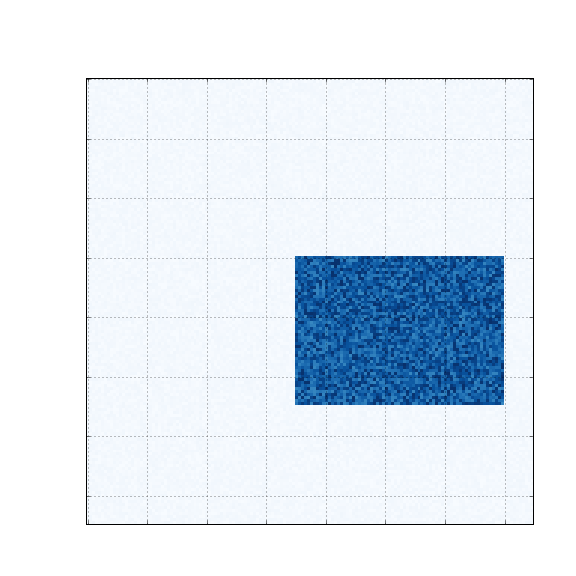
\includegraphics[width=\textwidth]{img/a-bic-structure.png}
          \caption{}
          \label{fig:bic-syntetic-structure:a}
      \end{subfigure}
      ~
      \begin{subfigure}[b]{0.16\textwidth}
          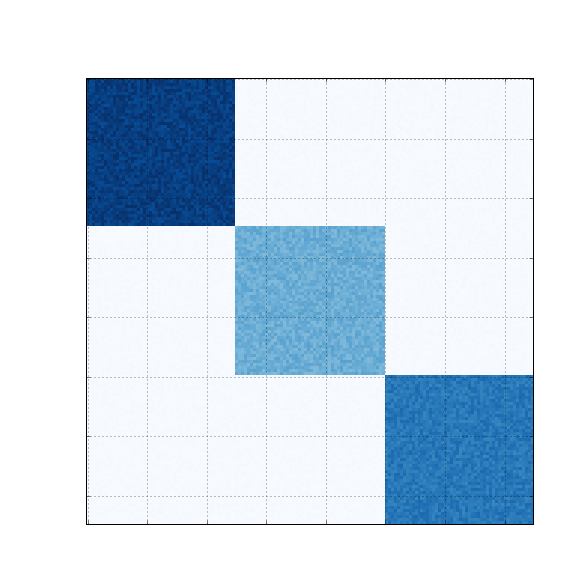
\includegraphics[width=\textwidth]{img/b-bic-structure.png}
          \caption{}
          \label{fig:bic-syntetic-structure:b}
      \end{subfigure}
      ~
      \begin{subfigure}[b]{0.16\textwidth}
          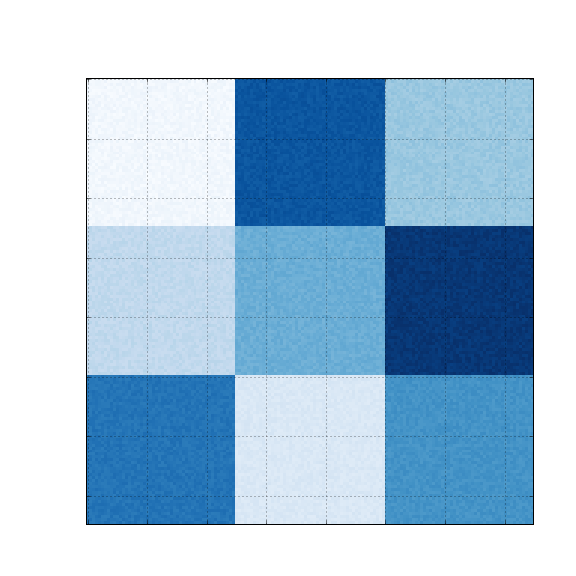
\includegraphics[width=\textwidth]{img/c-bic-structure.png}
          \caption{}
          \label{fig:bic-syntetic-structure:c}
      \end{subfigure}
      ~
      \begin{subfigure}[b]{0.16\textwidth}
          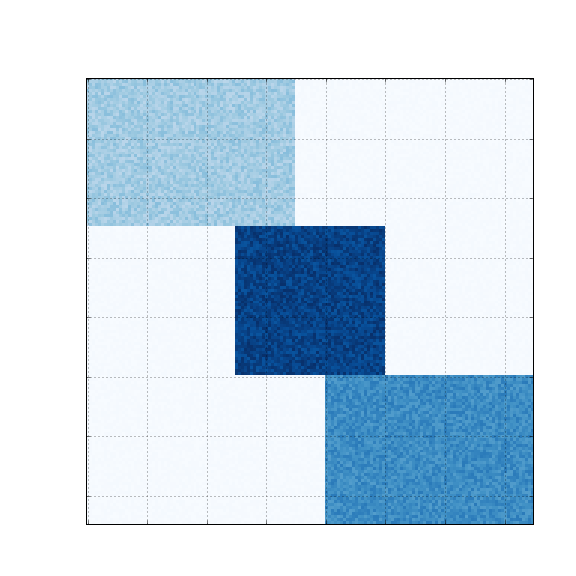
\includegraphics[width=\textwidth]{img/d-bic-structure.png}
          \caption{}
          \label{fig:bic-syntetic-structure:d}
      \end{subfigure}
      ~
      \begin{subfigure}[b]{0.16\textwidth}
          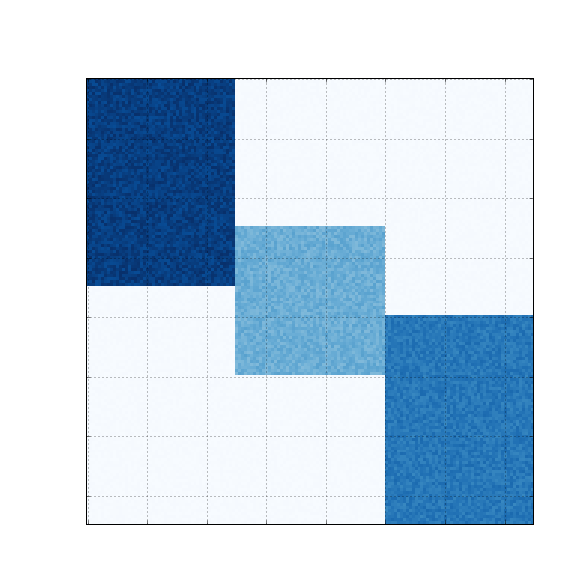
\includegraphics[width=\textwidth]{img/e-bic-structure.png}
          \caption{}
          \label{fig:bic-syntetic-structure:e}
      \end{subfigure}
      \label{fig:bic-syntetic-structure}
  \end{figure}

  % \[
  %     \begin{bmatrix}
  %         \mathbf{30,3} & \mathbf{31,6} & \mathbf{30,9} & 1,0           & 0,8           & 0,9           & 0,7           & 0,7           & 0,1           \\
  %         \mathbf{29,1} & \mathbf{30,7} & \mathbf{30,0} & 0,7           & 0,0           & 0,6           & 0,8           & 0,1           & 0,9           \\
  %         \mathbf{30,8} & \mathbf{29,5} & \mathbf{31,5} & 0,2           & 0,7           & 0,2           & 0,9           & 0,7           & 0,5           \\
  %         0,4           & 0,9           & 1,0           & \mathbf{10,5} & \mathbf{9,2}  & \mathbf{10,8} & 0,8           & 0,8           & 0,8           \\
  %         0,5           & 0,7           & 0,5           & \mathbf{11,1} & \mathbf{10,0} & \mathbf{9,2}  & 0,9           & 0,7           & 0,6           \\
  %         0,3           & 0,4           & 0,5           & \mathbf{10,8} & \mathbf{11,2} & \mathbf{10,9} & 0,5           & 0,3           & 0,1           \\
  %         0,0           & 0,7           & 0,4           & 0,4           & 0,1           & 0,4           & \mathbf{20,2} & \mathbf{19,6} & \mathbf{20,4} \\
  %         0,8           & 0,5           & 1,0           & 0,4           & 0,7           & 0,3           & \mathbf{21,2} & \mathbf{20,7} & \mathbf{19,4} \\
  %         0,0           & 0,6           & 0,4           & 0,6           & 0,1           & 0,1           & \mathbf{19,9} & \mathbf{20,2} & \mathbf{20,9}
  %     \end{bmatrix}
  % \]

\end{frame}

%------------------------------------------------

\begin{frame}
\frametitle{Reconstrução para as bases (a), (b) e (c)}

  % \begin{itemize}
  %   \item $k = 2$ para (a)
  %   \item $k = 3$ para (b), (c), (d) e (e)
  % \end{itemize}

%   \begin{minipage}{0.2\textwidth}
%     \begin{itemize}
%         \setlength\itemsep{1em}
%         \item Original
%         \item \textit{k-means}
%         \item \textit{fuzzy k-means}
%         \item \textit{ONMTF}
%         \item \textit{FNMTF}
%         \item \textit{OvNMTF}
%         \item \textit{BinOvNMTF}
%     \end{itemize}
% \end{minipage}
% \begin{minipage}{0.75\textwidth}
    % \rule{\textwidth}{0.75\textwidth}


  \begin{figure}[H]
  \centering
      \begin{subfigure}[b]{0.13\textwidth}
          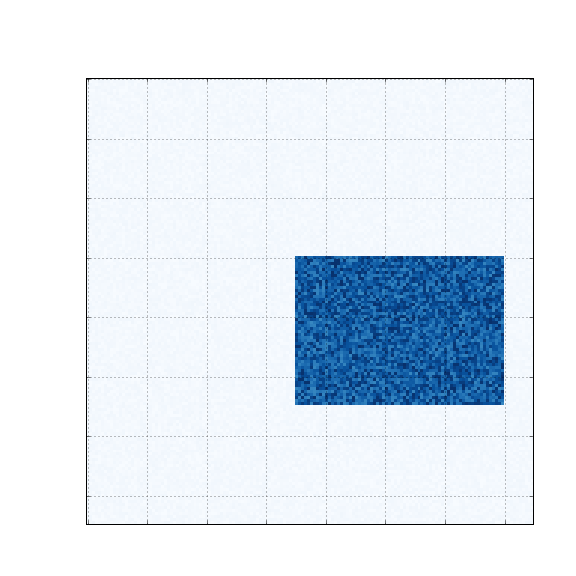
\includegraphics[width=\textwidth]{img/a-bic-structure.png}
      \end{subfigure}
      \begin{subfigure}[b]{0.13\textwidth}
          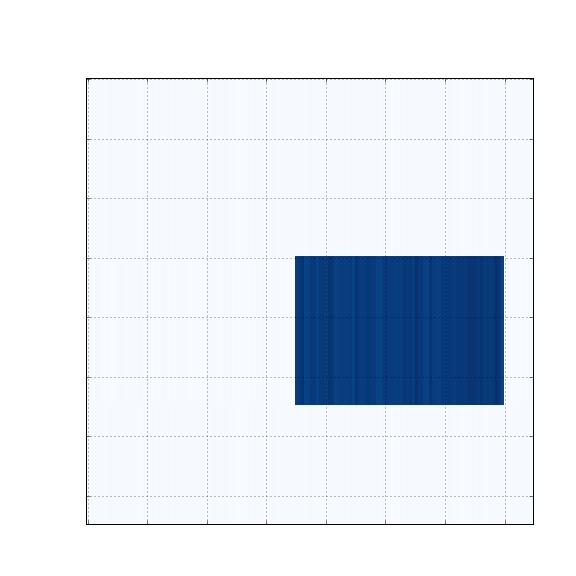
\includegraphics[width=\textwidth]{img/a-reconstruction-kmeans.png}
      \end{subfigure}
      \begin{subfigure}[b]{0.13\textwidth}
          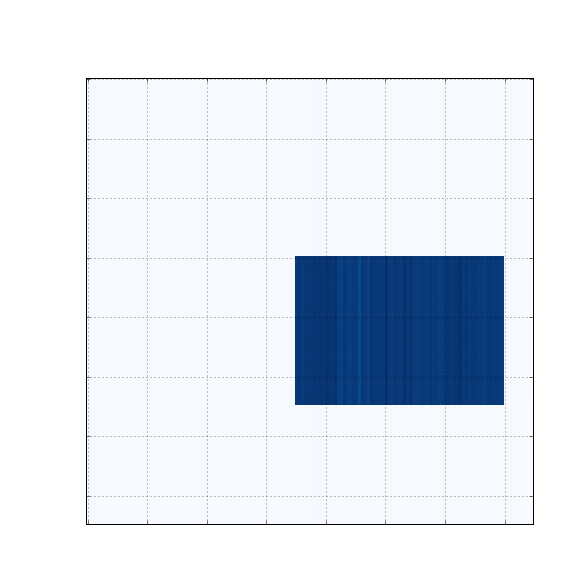
\includegraphics[width=\textwidth]{img/a-reconstruction-fkmeans.png}
      \end{subfigure}
      \begin{subfigure}[b]{0.13\textwidth}
          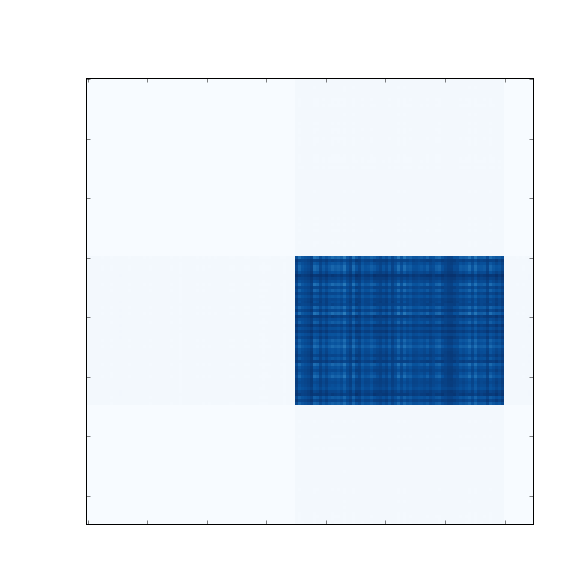
\includegraphics[width=\textwidth]{img/a-reconstruction-onmtf.png}
      \end{subfigure}
      \begin{subfigure}[b]{0.13\textwidth}
          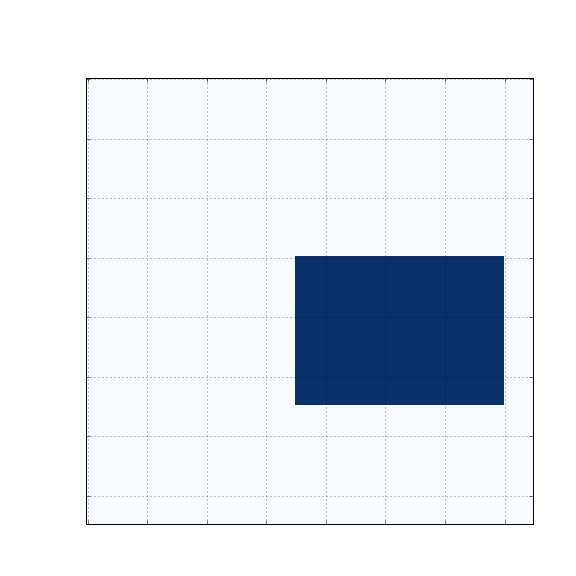
\includegraphics[width=\textwidth]{img/a-reconstruction-fnmtf.png}
      \end{subfigure}
      \begin{subfigure}[b]{0.13\textwidth}
          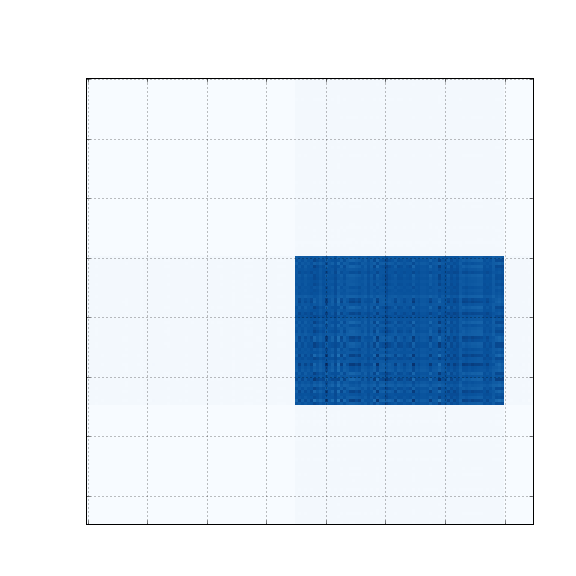
\includegraphics[width=\textwidth]{img/a-reconstruction-ovnmtf.png}
      \end{subfigure}
      \begin{subfigure}[b]{0.13\textwidth}
          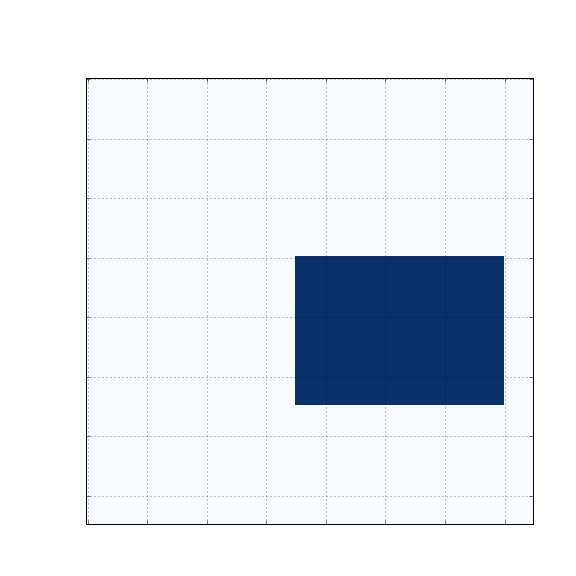
\includegraphics[width=\textwidth]{img/a-reconstruction-binovnmtf.png}
      \end{subfigure}

      \begin{subfigure}[b]{0.13\textwidth}
          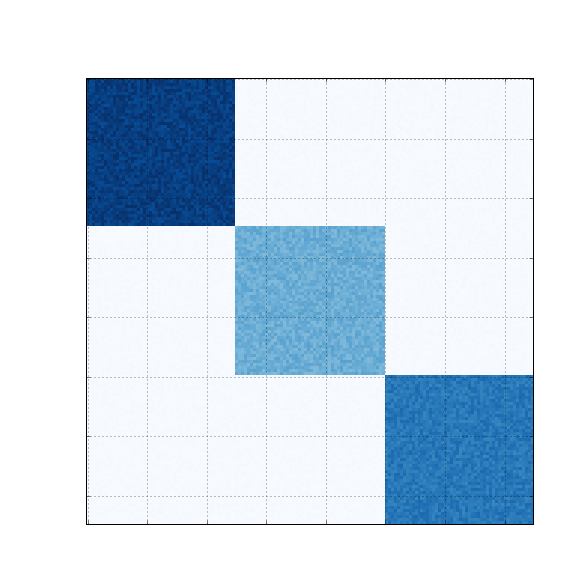
\includegraphics[width=\textwidth]{img/b-bic-structure.png}
      \end{subfigure}
      \begin{subfigure}[b]{0.13\textwidth}
          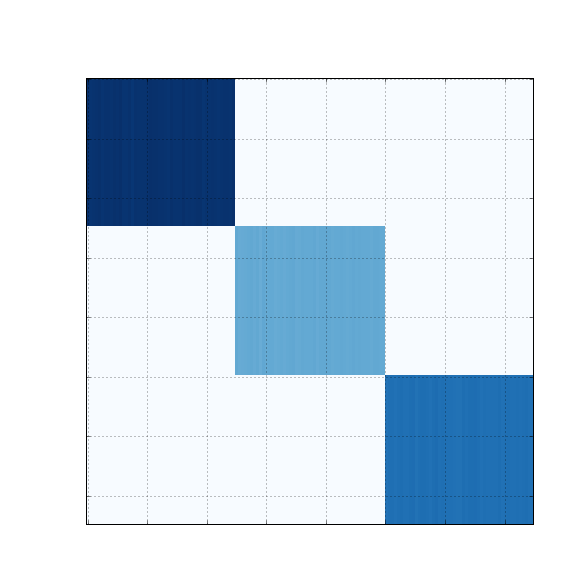
\includegraphics[width=\textwidth]{img/b-reconstruction-kmeans.png}
      \end{subfigure}
      \begin{subfigure}[b]{0.13\textwidth}
          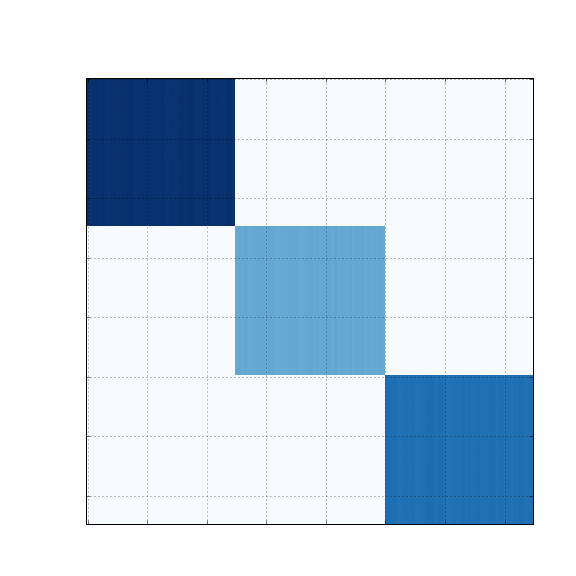
\includegraphics[width=\textwidth]{img/b-reconstruction-fkmeans.png}
      \end{subfigure}
      \begin{subfigure}[b]{0.13\textwidth}
          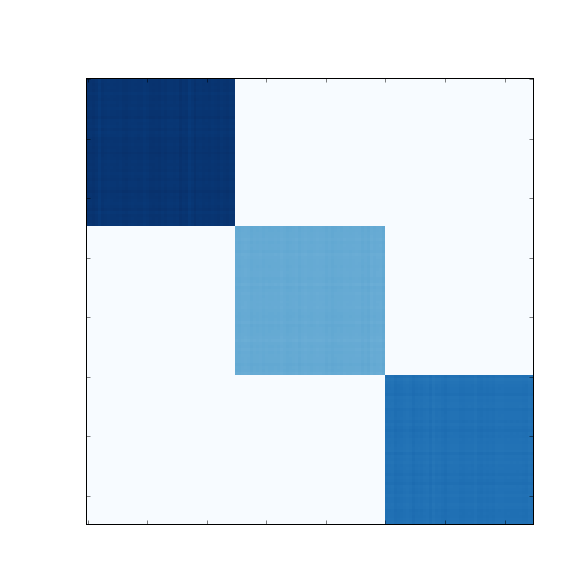
\includegraphics[width=\textwidth]{img/b-reconstruction-onmtf.png}
      \end{subfigure}
      \begin{subfigure}[b]{0.13\textwidth}
          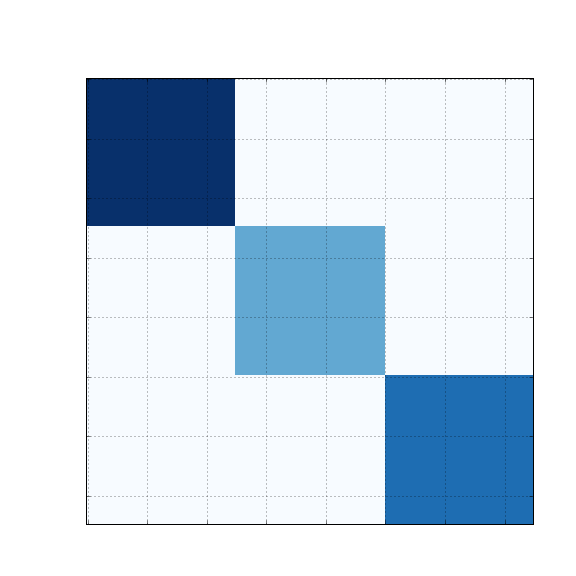
\includegraphics[width=\textwidth]{img/b-reconstruction-fnmtf.png}
      \end{subfigure}
      \begin{subfigure}[b]{0.13\textwidth}
          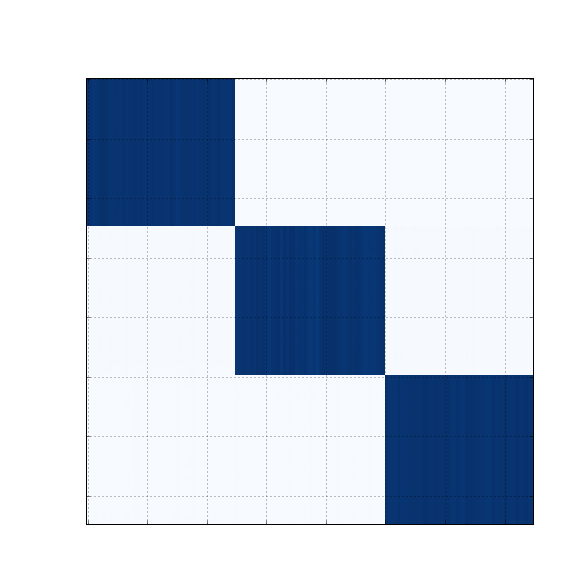
\includegraphics[width=\textwidth]{img/b-reconstruction-ovnmtf.png}
      \end{subfigure}
      \begin{subfigure}[b]{0.13\textwidth}
          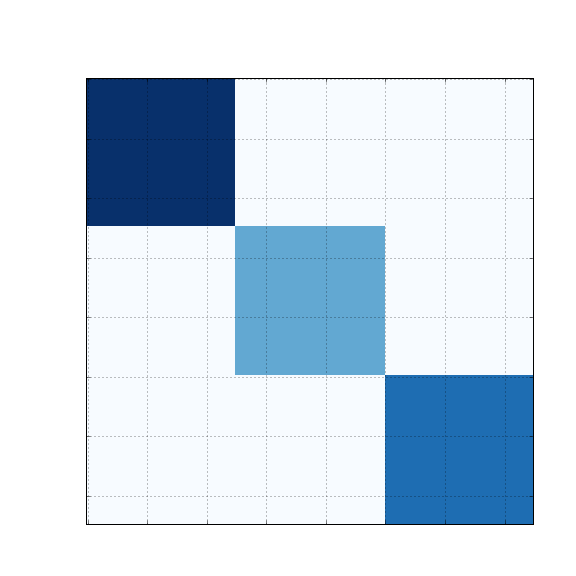
\includegraphics[width=\textwidth]{img/b-reconstruction-binovnmtf.png}
      \end{subfigure}

      \begin{subfigure}[b]{0.13\textwidth}
          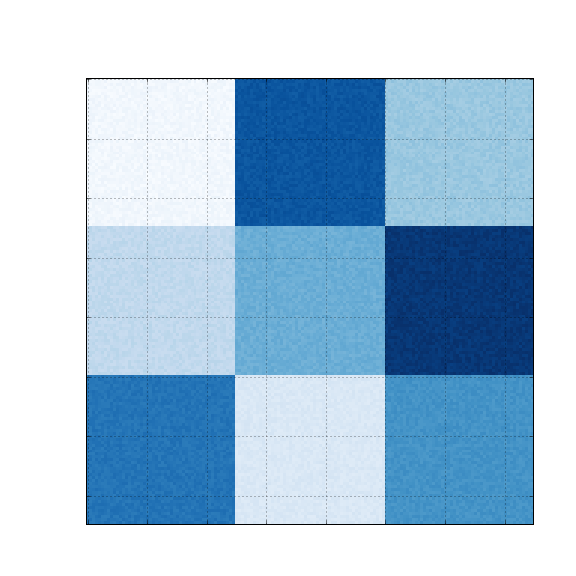
\includegraphics[width=\textwidth]{img/c-bic-structure.png}
          \caption*{original}
      \end{subfigure}
      \begin{subfigure}[b]{0.13\textwidth}
          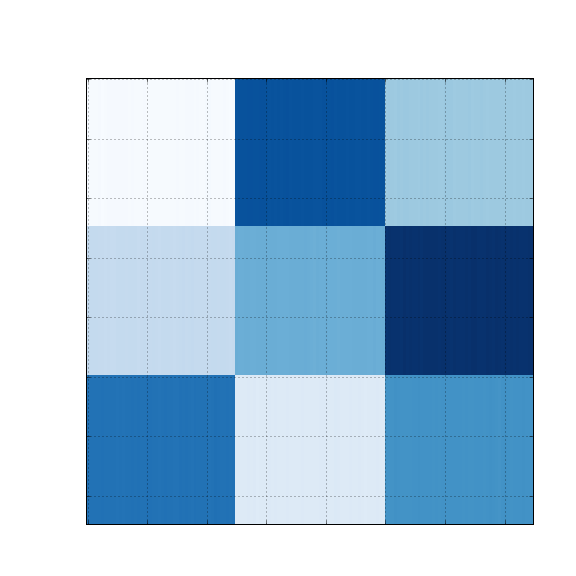
\includegraphics[width=\textwidth]{img/c-reconstruction-kmeans.png}
          \caption*{kmeans}
      \end{subfigure}
      \begin{subfigure}[b]{0.13\textwidth}
          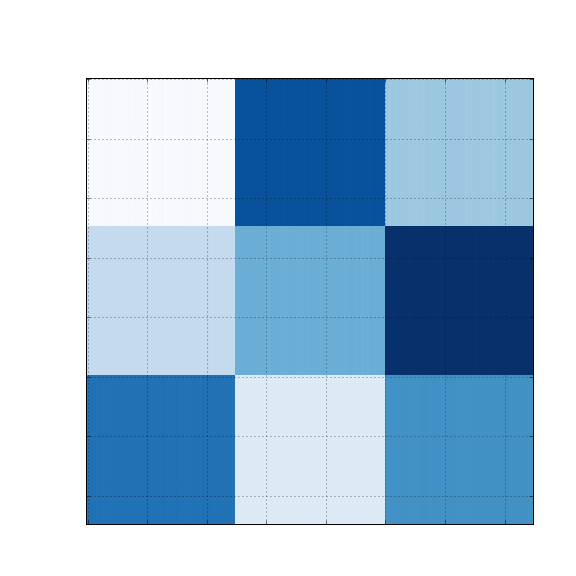
\includegraphics[width=\textwidth]{img/c-reconstruction-fkmeans.png}
          \caption*{fkmeans}
      \end{subfigure}
      \begin{subfigure}[b]{0.13\textwidth}
          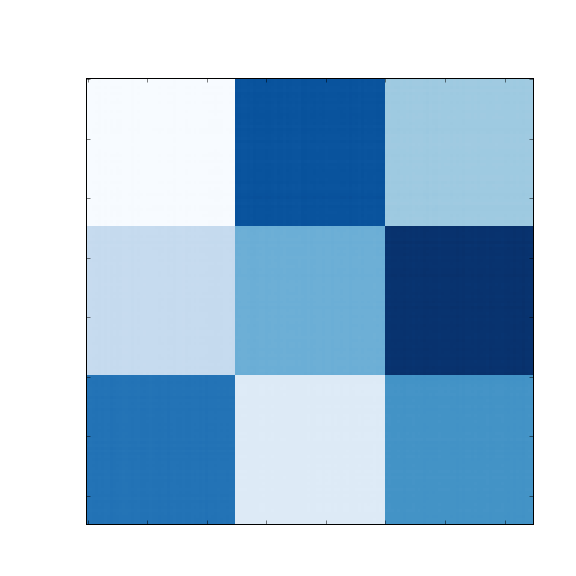
\includegraphics[width=\textwidth]{img/c-reconstruction-onmtf.png}
          \caption*{ONTMF}
      \end{subfigure}
      \begin{subfigure}[b]{0.13\textwidth}
          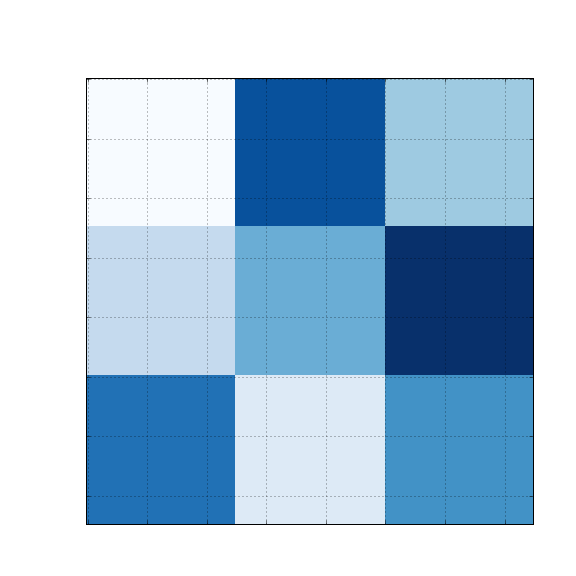
\includegraphics[width=\textwidth]{img/c-reconstruction-fnmtf.png}
          \caption*{FNMTF}
      \end{subfigure}
      \begin{subfigure}[b]{0.13\textwidth}
          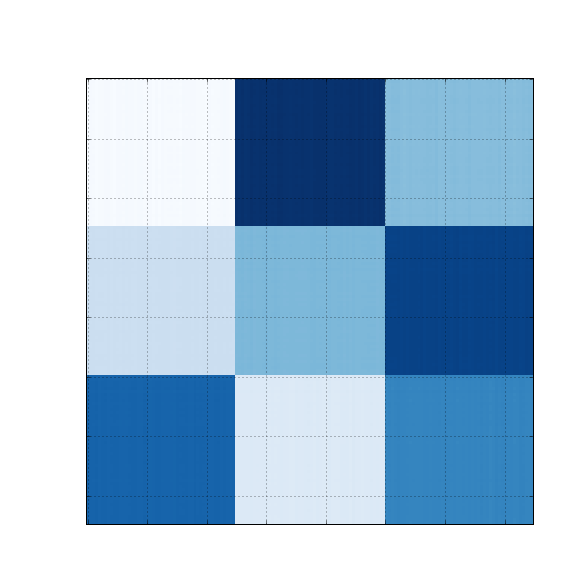
\includegraphics[width=\textwidth]{img/c-reconstruction-ovnmtf.png}
          \caption*{OvNMTF}
      \end{subfigure}
      \begin{subfigure}[b]{0.13\textwidth}
          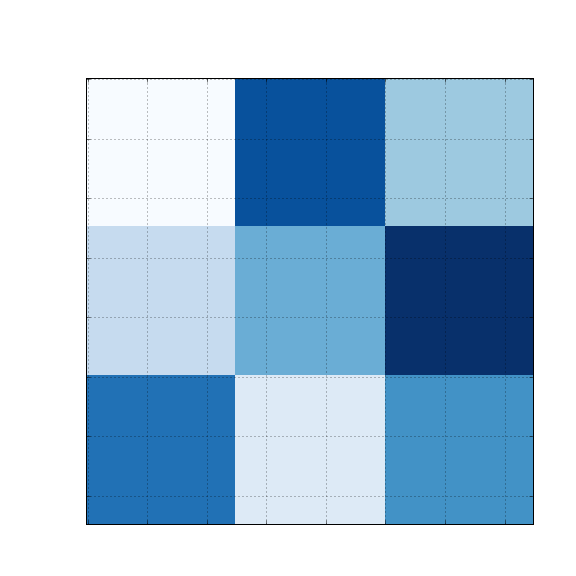
\includegraphics[width=\textwidth]{img/c-reconstruction-binovnmtf.png}
          \caption*{BOvNMTF}
      \end{subfigure}
  \end{figure}
  % \end{minipage}
\end{frame}

\begin{frame}
\frametitle{Reconstrução para as bases (d) e (e)}

  \begin{itemize}
    % \item Parâmetros:
    % \begin{itemize}
      % \item $t_{max} = 1000$
      % \item diferença do erro de quantização em duas iterações consecutivas ($\leq 1 \times 10^{-4}$)
      \item $k = l = 3$ (\textit{kmeans}, \textit{fkmeans}, \textit{ONMTF} e \textit{FNMTF})
      \item $k = 3$ e $l = 2$ (\textit{OvNMTF} e \textit{BinOvNMTF})
    % \end{itemize}
  \end{itemize}

  \begin{figure}[H]
  \centering
      \begin{subfigure}[b]{0.13\textwidth}
          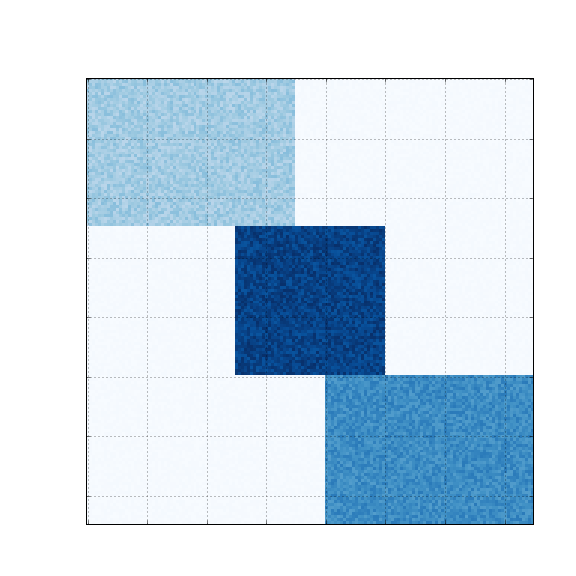
\includegraphics[width=\textwidth]{img/d-bic-structure.png}
      \end{subfigure}
      \begin{subfigure}[b]{0.13\textwidth}
          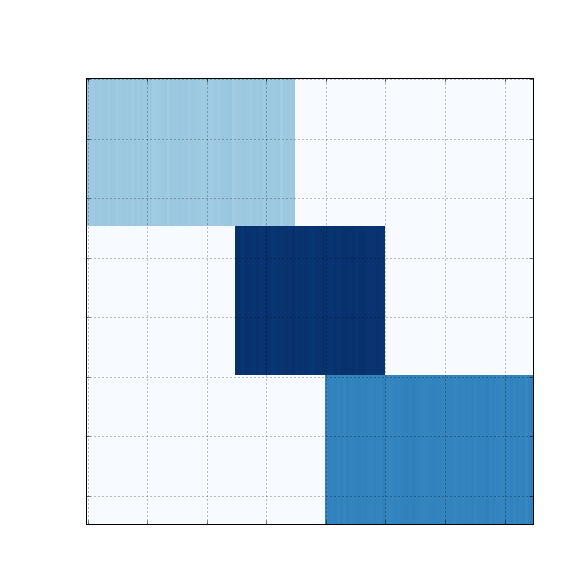
\includegraphics[width=\textwidth]{img/d-reconstruction-kmeans.png}
      \end{subfigure}
      \begin{subfigure}[b]{0.13\textwidth}
          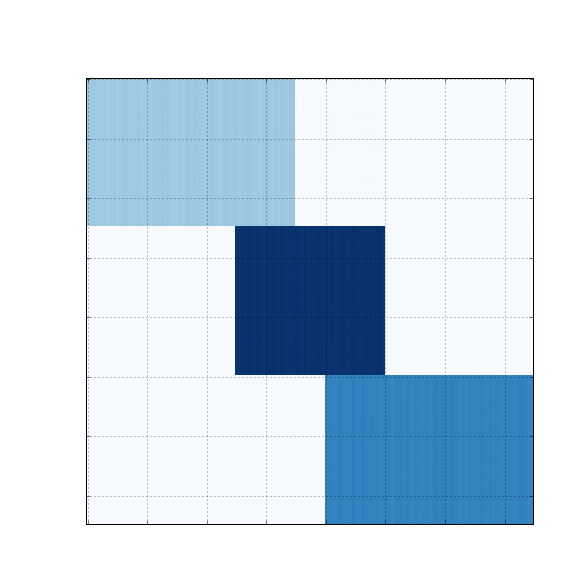
\includegraphics[width=\textwidth]{img/d-reconstruction-fkmeans.png}
      \end{subfigure}
      \begin{subfigure}[b]{0.13\textwidth}
          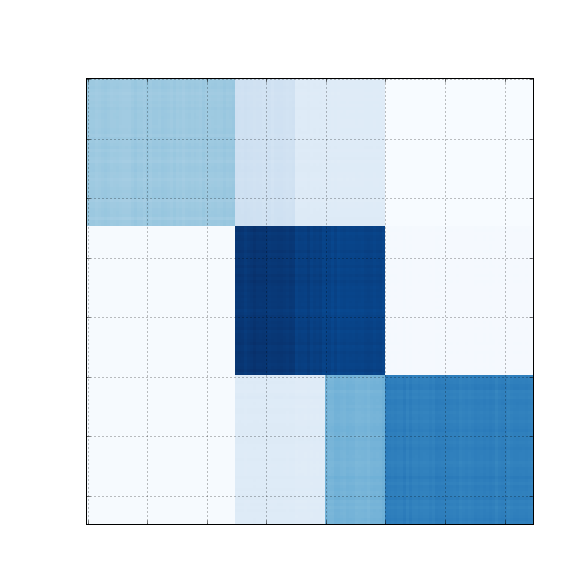
\includegraphics[width=\textwidth]{img/d-reconstruction-onmtf.png}
      \end{subfigure}
      \begin{subfigure}[b]{0.13\textwidth}
          \includegraphics[width=\textwidth]{img/d-reconstruction-fnmtf.png}
      \end{subfigure}
      \begin{subfigure}[b]{0.13\textwidth}
          \includegraphics[width=\textwidth]{img/d-reconstruction-ovnmtf.png}
      \end{subfigure}
      \begin{subfigure}[b]{0.13\textwidth}
          \includegraphics[width=\textwidth]{img/d-reconstruction-binovnmtf.png}
      \end{subfigure}

      \begin{subfigure}[b]{0.13\textwidth}
          \includegraphics[width=\textwidth]{img/e-bic-structure.png}
          \caption*{original}
      \end{subfigure}
      \begin{subfigure}[b]{0.13\textwidth}
          \includegraphics[width=\textwidth]{img/e-reconstruction-kmeans.png}
          \caption*{kmeans}
      \end{subfigure}
      \begin{subfigure}[b]{0.13\textwidth}
          \includegraphics[width=\textwidth]{img/e-reconstruction-fkmeans.png}
          \caption*{fkmeans}
      \end{subfigure}
      \begin{subfigure}[b]{0.13\textwidth}
          \includegraphics[width=\textwidth]{img/e-reconstruction-onmtf.png}
          \caption*{ONTMF}
      \end{subfigure}
      \begin{subfigure}[b]{0.13\textwidth}
          \includegraphics[width=\textwidth]{img/e-reconstruction-fnmtf.png}
          \caption*{FNMTF}
      \end{subfigure}
      \begin{subfigure}[b]{0.13\textwidth}
          \includegraphics[width=\textwidth]{img/e-reconstruction-ovnmtf.png}
          \caption*{OvNMTF}
      \end{subfigure}
      \begin{subfigure}[b]{0.13\textwidth}
          \includegraphics[width=\textwidth]{img/e-reconstruction-binovnmtf.png}
          \caption*{BOvNMTF}
      \end{subfigure}
  \end{figure}

\end{frame}


%------------------------------------------------


\begin{frame}
\frametitle{Reconstrução a partir dos resultados do algoritmo \textit{k-means} e \textit{fuzzy k-means}}
\begin{itemize}
  \item $k = 5$ para (e)
\end{itemize}
  % Resultado da reconstrução da base de dados (e) ($k = 5$)
  \begin{figure}[H]
  \centering
      % \caption{Resultado da reconstrução da base de dados (e) utilizando o algoritmo \textit{k-means} com $k = 5$.}
      \begin{subfigure}[b]{0.3\textwidth}
          % \includegraphics[width=\textwidth]{img/e-reconstruction-fkmeans.png}
          \includegraphics[width=\textwidth]{img/e-reconstruction-2-kmeans.png}
          \caption*{k-means}
      \end{subfigure}
      \begin{subfigure}[b]{0.3\textwidth}
          % \includegraphics[width=\textwidth]{img/e-reconstruction-fkmeans.png}
          \includegraphics[width=\textwidth]{img/e-reconstruction-2-fkmeans.png}
          \caption*{fuzzy k-means}
      \end{subfigure}
  \end{figure}

  % \begin{figure}[H]
  % \centering
  %     % \caption{Resultado da reconstrução da base de dados (e) utilizando o algoritmo \textit{fuzzy k-means} com $k = 5$.}
  %     \includegraphics[width=0.3\textwidth]{img/e-reconstruction-2-fkmeans.png}
  % \end{figure}

\end{frame}

%------------------------------------------------

% \begin{frame} [allowframebreaks]
% \frametitle{Reconstrução a partir dos resultados do algoritmo \textit{fuzzy k-means}}

%   \begin{itemize}
%     \item Parâmetros:
%     \begin{itemize}
%       \item $t_{max} = 300$
%       \item diferença do erro de quantização em duas iterações consecutivas ($\leq 1 \times 10^{-4}$)
%       \item $k = 2$ para (a) e $k = 3$ para (b), (c), (d) e (e)
%       \item $w = 2$
%     \end{itemize}
%   \end{itemize}

%   \begin{figure}[H]
%   \centering
%       \begin{subfigure}[b]{0.16\textwidth}
%           \includegraphics[width=\textwidth]{img/a-bic-structure.png}
%       \end{subfigure}
%       \begin{subfigure}[b]{0.16\textwidth}
%           \includegraphics[width=\textwidth]{img/b-bic-structure.png}
%       \end{subfigure}
%       \begin{subfigure}[b]{0.16\textwidth}
%           \includegraphics[width=\textwidth]{img/c-bic-structure.png}
%       \end{subfigure}
%       \begin{subfigure}[b]{0.16\textwidth}
%           \includegraphics[width=\textwidth]{img/d-bic-structure.png}
%       \end{subfigure}
%       \begin{subfigure}[b]{0.16\textwidth}
%           \includegraphics[width=\textwidth]{img/e-bic-structure.png}
%       \end{subfigure}

%       \begin{subfigure}[b]{0.16\textwidth}
%           \includegraphics[width=\textwidth]{img/a-reconstruction-fkmeans.png}
%           \caption{}
%       \end{subfigure}
%       \begin{subfigure}[b]{0.16\textwidth}
%           \includegraphics[width=\textwidth]{img/b-reconstruction-fkmeans.png}
%           \caption{}
%       \end{subfigure}
%       \begin{subfigure}[b]{0.16\textwidth}
%           \includegraphics[width=\textwidth]{img/c-reconstruction-fkmeans.png}
%           \caption{}
%       \end{subfigure}
%       \begin{subfigure}[b]{0.16\textwidth}
%           \includegraphics[width=\textwidth]{img/d-reconstruction-fkmeans.png}
%           \caption{}
%       \end{subfigure}
%       \begin{subfigure}[b]{0.16\textwidth}
%           \includegraphics[width=\textwidth]{img/e-reconstruction-fkmeans.png}
%           \caption{}
%       \end{subfigure}
%   \end{figure}

%   \begin{figure}[H]
%   \centering
%       \caption{Resultado da reconstrução da base de dados (e) utilizando o algoritmo \textit{fuzzy k-means} com $k = 5$.}
%       \includegraphics[width=0.3\textwidth]{img/e-reconstruction-2-fkmeans.png}
%   \end{figure}

% \end{frame}

%------------------------------------------------

% \begin{frame}
% \frametitle{Reconstrução a partir dos resultados do algoritmo \textit{ONMTF} e \textit{FNMTF} I}

%   \begin{itemize}
%     \item Parâmetros:
%     \begin{itemize}
%       \item $k = l = 2$ para (a) e $k = l = 3$ para (b), (c), (d) e (e)
%     \end{itemize}
%   \end{itemize}

%   \begin{figure}[H]
%   \centering
%       \begin{subfigure}[b]{0.16\textwidth}
%           \includegraphics[width=\textwidth]{img/a-bic-structure.png}
%       \end{subfigure}
%       \begin{subfigure}[b]{0.16\textwidth}
%           \includegraphics[width=\textwidth]{img/b-bic-structure.png}
%       \end{subfigure}
%       \begin{subfigure}[b]{0.16\textwidth}
%           \includegraphics[width=\textwidth]{img/c-bic-structure.png}
%       \end{subfigure}
%       \begin{subfigure}[b]{0.16\textwidth}
%           \includegraphics[width=\textwidth]{img/d-bic-structure.png}
%       \end{subfigure}
%       \begin{subfigure}[b]{0.16\textwidth}
%           \includegraphics[width=\textwidth]{img/e-bic-structure.png}
%       \end{subfigure}

%       \begin{subfigure}[b]{0.16\textwidth}
%           \includegraphics[width=\textwidth]{img/a-reconstruction-onmtf.png}
%           \caption{}
%       \end{subfigure}
%       \begin{subfigure}[b]{0.16\textwidth}
%           \includegraphics[width=\textwidth]{img/b-reconstruction-onmtf.png}
%           \caption{}
%       \end{subfigure}
%       \begin{subfigure}[b]{0.16\textwidth}
%           \includegraphics[width=\textwidth]{img/c-reconstruction-onmtf.png}
%           \caption{}
%       \end{subfigure}
%       \begin{subfigure}[b]{0.16\textwidth}
%           \includegraphics[width=\textwidth]{img/d-reconstruction-onmtf.png}
%           \caption{}
%       \end{subfigure}
%       \begin{subfigure}[b]{0.16\textwidth}
%           \includegraphics[width=\textwidth]{img/e-reconstruction-onmtf.png}
%               \caption{}
%       \end{subfigure}

%       \begin{subfigure}[b]{0.16\textwidth}
%           \includegraphics[width=\textwidth]{img/a-reconstruction-fnmtf.png}
%           \caption{}
%       \end{subfigure}
%       \begin{subfigure}[b]{0.16\textwidth}
%           \includegraphics[width=\textwidth]{img/b-reconstruction-fnmtf.png}
%           \caption{}
%       \end{subfigure}
%       \begin{subfigure}[b]{0.16\textwidth}
%           \includegraphics[width=\textwidth]{img/c-reconstruction-fnmtf.png}
%           \caption{}
%       \end{subfigure}
%       \begin{subfigure}[b]{0.16\textwidth}
%           \includegraphics[width=\textwidth]{img/d-reconstruction-fnmtf.png}
%           \caption{}
%       \end{subfigure}
%       \begin{subfigure}[b]{0.16\textwidth}
%           \includegraphics[width=\textwidth]{img/e-reconstruction-fnmtf.png}
%               \caption{}
%       \end{subfigure}
%   \end{figure}
% \end{frame}

\begin{frame}
\frametitle{Reconstrução a partir dos resultados do algoritmo \textit{ONMTF} e \textit{FNMTF}}

  \begin{itemize}
    \item $k = 5$ para (d)
    \item $l = 5$ para (e)
  \end{itemize}

  \begin{figure}[H]
  \centering
      % \caption{
      %     Resultado da reconstrução da base de dados (d) com $k = 5$ e (e) com $l = 5$, respectivamente, utilizando o algoritmo \textit{ONMTF}.
      % }
      \begin{subfigure}[b]{0.2\textwidth}
          \includegraphics[width=\textwidth]{img/d-bic-structure.png}
      \end{subfigure}
      \begin{subfigure}[b]{0.2\textwidth}
          \includegraphics[width=\textwidth]{img/d-reconstruction-2-onmtf.png}
      \end{subfigure}
      \begin{subfigure}[b]{0.2\textwidth}
          \includegraphics[width=\textwidth]{img/d-reconstruction-2-fnmtf.png}
      \end{subfigure}

      \begin{subfigure}[b]{0.2\textwidth}
          \includegraphics[width=\textwidth]{img/e-bic-structure.png}
          \caption*{original}
      \end{subfigure}
      \begin{subfigure}[b]{0.2\textwidth}
          \includegraphics[width=\textwidth]{img/e-reconstruction-2-onmtf.png}
          \caption*{ONTMF}
      \end{subfigure}
      \begin{subfigure}[b]{0.2\textwidth}
          \includegraphics[width=\textwidth]{img/e-reconstruction-2-fnmtf.png}
          \caption*{FNMTF}
      \end{subfigure}
  \end{figure}

  % \begin{figure}[H]
  % \centering
  %     % \caption{
  %     %     Resultado da reconstrução da base de dados (d) com $k = 5$ e (e) com $l = 5$, respectivamente, utilizando o algoritmo \textit{FNMTF}.
  %     % }
  %     \begin{subfigure}[b]{0.3\textwidth}
  %         \includegraphics[width=\textwidth]{img/d-reconstruction-2-fnmtf.png}
  %     \end{subfigure}
  %     \begin{subfigure}[b]{0.3\textwidth}
  %         \includegraphics[width=\textwidth]{img/e-reconstruction-2-fnmtf.png}
  %     \end{subfigure}
  % \end{figure}

\end{frame}

%------------------------------------------------

% \begin{frame} [allowframebreaks]
% \frametitle{Reconstrução a partir dos resultados do algoritmo \textit{FNMTF}}

%   \begin{itemize}
%     \item Parâmetros:
%     \begin{itemize}
%       \item $t_{max} = 300$
%       \item diferença do erro de quantização em duas iterações consecutivas ($\leq 1 \times 10^{-4}$)
%       \item $k = l = 2$ para (a) e $k = l = 3$ para (b), (c), (d) e (e)
%     \end{itemize}
%   \end{itemize}

%   \begin{figure}[H]
%   \centering
%       \begin{subfigure}[b]{0.16\textwidth}
%           \includegraphics[width=\textwidth]{img/a-bic-structure.png}
%       \end{subfigure}
%       \begin{subfigure}[b]{0.16\textwidth}
%           \includegraphics[width=\textwidth]{img/b-bic-structure.png}
%       \end{subfigure}
%       \begin{subfigure}[b]{0.16\textwidth}
%           \includegraphics[width=\textwidth]{img/c-bic-structure.png}
%       \end{subfigure}
%       \begin{subfigure}[b]{0.16\textwidth}
%           \includegraphics[width=\textwidth]{img/d-bic-structure.png}
%       \end{subfigure}
%       \begin{subfigure}[b]{0.16\textwidth}
%           \includegraphics[width=\textwidth]{img/e-bic-structure.png}
%       \end{subfigure}

%       \begin{subfigure}[b]{0.16\textwidth}
%           \includegraphics[width=\textwidth]{img/a-reconstruction-fnmtf.png}
%           \caption{}
%       \end{subfigure}
%       \begin{subfigure}[b]{0.16\textwidth}
%           \includegraphics[width=\textwidth]{img/b-reconstruction-fnmtf.png}
%           \caption{}
%       \end{subfigure}
%       \begin{subfigure}[b]{0.16\textwidth}
%           \includegraphics[width=\textwidth]{img/c-reconstruction-fnmtf.png}
%           \caption{}
%       \end{subfigure}
%       \begin{subfigure}[b]{0.16\textwidth}
%           \includegraphics[width=\textwidth]{img/d-reconstruction-fnmtf.png}
%           \caption{}
%       \end{subfigure}
%       \begin{subfigure}[b]{0.16\textwidth}
%           \includegraphics[width=\textwidth]{img/e-reconstruction-fnmtf.png}
%               \caption{}
%       \end{subfigure}
%   \end{figure}

%   \begin{figure}[H]
%   \centering
%       \caption{
%           Resultado da reconstrução da base de dados (d) com $k = 5$ e (e) com $l = 5$, respectivamente, utilizando o algoritmo \textit{FNMTF}.
%       }
%       \begin{subfigure}[b]{0.3\textwidth}
%           \includegraphics[width=\textwidth]{img/d-reconstruction-2-fnmtf.png}
%       \end{subfigure}
%       \begin{subfigure}[b]{0.3\textwidth}
%           \includegraphics[width=\textwidth]{img/e-reconstruction-2-fnmtf.png}
%       \end{subfigure}
%   \end{figure}

% \end{frame}

%------------------------------------------------

% \begin{frame} [allowframebreaks]
% \frametitle{Reconstrução a partir dos resultados do algoritmo \textit{BinOvNMTF}}

%   \begin{itemize}
%     % \item Parâmetros:
%     % \begin{itemize}
%       % \item $t_{max} = 300$
%       % \item diferença do erro de quantização em duas iterações consecutivas ($\leq 1 \times 10^{-4}$)
%       \item $k = l = 2$ para (a), $k = 3$ e $l = 2$ para (b), (d) e (e), e $k = l = 3$ para (c)
%     % \end{itemize}
%   \end{itemize}

%   \begin{figure}[H]
%   \centering
%       \begin{subfigure}[b]{0.16\textwidth}
%           \includegraphics[width=\textwidth]{img/a-bic-structure.png}
%       \end{subfigure}
%       \begin{subfigure}[b]{0.16\textwidth}
%           \includegraphics[width=\textwidth]{img/b-bic-structure.png}
%       \end{subfigure}
%       \begin{subfigure}[b]{0.16\textwidth}
%           \includegraphics[width=\textwidth]{img/c-bic-structure.png}
%       \end{subfigure}
%       \begin{subfigure}[b]{0.16\textwidth}
%           \includegraphics[width=\textwidth]{img/d-bic-structure.png}
%       \end{subfigure}
%       \begin{subfigure}[b]{0.16\textwidth}
%           \includegraphics[width=\textwidth]{img/e-bic-structure.png}
%       \end{subfigure}

%       \begin{subfigure}[b]{0.16\textwidth}
%           \includegraphics[width=\textwidth]{img/a-reconstruction-binovnmtf.png}
%           \caption{}
%       \end{subfigure}
%       \begin{subfigure}[b]{0.16\textwidth}
%           \includegraphics[width=\textwidth]{img/b-reconstruction-binovnmtf.png}
%           \caption{}
%       \end{subfigure}
%       \begin{subfigure}[b]{0.16\textwidth}
%           \includegraphics[width=\textwidth]{img/c-reconstruction-binovnmtf.png}
%           \caption{}
%       \end{subfigure}
%       \begin{subfigure}[b]{0.16\textwidth}
%           \includegraphics[width=\textwidth]{img/d-reconstruction-binovnmtf.png}
%           \caption{}
%       \end{subfigure}
%       \begin{subfigure}[b]{0.16\textwidth}
%           \includegraphics[width=\textwidth]{img/e-reconstruction-binovnmtf.png}
%               \caption{}
%       \end{subfigure}
%   \end{figure}

\begin{frame}
\frametitle{Reconstrução a partir dos resultados do algoritmo \textit{BinOvNMTF}}

  \begin{itemize}
    \item $k = 5$ para (e)
  \end{itemize}

  \begin{figure}[H]
  \centering
      % \caption{Resultado da reconstrução da base de dados (e) utilizando o algoritmo \textit{Bin\-OvNMTF} com $k = 5$.}
      \includegraphics[width=0.3\textwidth]{img/e-reconstruction-2-binovnmtf.png}
  \end{figure}

\end{frame}


%------------------------------------------------

\begin{frame}
\frametitle{Análise da capacidade de quantização}

  \begin{table}[H]
  \centering
      \resizebox{\linewidth}{!}{\begin{tabular}{lccccc}
          \hline
          & \textbf{base (a)} & \textbf{base (b)} & \textbf{base (c)} & \textbf{base (d)} & \textbf{base (e)} \\
          \hline
          \textit{k-means}        & $30.336,0$ & $62.776,5$ & $184.992,8$ & $\mathbf{79.238,5}$  & $2.886.245,5$        \\

          \textit{fuzzy k-means}  & $29.402,8$ & $63.768,5$ & $183.991,4$ & $\mathbf{78.340,0}$  & $2.307.168,6$        \\

         % \textit{BVD}            & $29.260,7$ & $61.536,5$ & $179.804,0$ & $\mathbf{75.575,0}$  & $\mathbf{77.135,5}$  \\

          \textit{ONMTF}          & $30.555,4$ & $60.794,8$ & $184.255,9$ & $579.136,7$          & $781.131,6$          \\

          \textit{FNMTF}          & $30.924,7$ & $64.636,1$ & $186.224,4$ & $1.634.328,5$        & $2.881.172,0$        \\

          \textit{OvNMTF}         & $30.439,8$ & $61.863,2$ & $178.886,8$ & $\mathbf{75.533,6}$  & $\mathbf{75.931,2}$  \\

          \textit{BinOvNMTF}      & $31.239,0$ & $63.660,4$ & $187.579,8$ & $\mathbf{79.968,0}$  & $3.160.391,0$        \\
          \hline \\
      \end{tabular}
      }
  \end{table}

  \begin{itemize}
    \item \textit{OvNMTF} preserva informação de sobreposição
    \item \textit{BinOvNMTF} preserva informação de sobreposição de colunas (d)
    \item \textit{ONMTF} preserva parte da informação de sobreposição
  \end{itemize}

\end{frame}

%------------------------------------------------

\begin{frame} [shrink=15]
\frametitle{Experimentos com bases de dados reais}

  Bases de dados
  \begin{itemize}
    \item \textit{NIPS}
    \begin{itemize}
      \item Trabalhos acadêmicos do período de 2001 a 2003
      \item Rotulados por áreas técnicas de forma desbalanceada
      \item Foram usadas $9$ das $13$ áreas técnicas
    \end{itemize}
    \item \textit{IG}
    \begin{itemize}
      \item Notícias publicadas no período de $2$ de janeiro de $2012$ à $11$ de outubro de $2014$
      \item Rotulados por canal que compreende o assunto da notícia
      \item Notícias distribuídas em $13$ canais de forma desbalanceada
      \item Notícias com mais de $200$ caracteres no corpo
    \end{itemize}
  \end{itemize}


  \begin{table}[h]
      \centering
      % \caption{Estatísticas das bases de dados usadas nos experimentos.}
      \resizebox{\linewidth}{!}{\begin{tabular}{lccccc}
          \hline
          \textbf{Base}     & \textbf{\# Palavras} & \textbf{\# Total de} & \textbf{\# Documentos} & \textbf{\# Grupos} & \textbf{Esparsidade} \\
          \textbf{de dados} & \textbf{únicas}      & \textbf{palavras}    &               &           &             \\
          \hline
          $\text{\textit{NIPS14-17}}$ & $6.881$  & $746.826$   & $555$   & $9$  & $0,804$ \\
          $\text{\textit{IG}}$        & $19.563$ & $1.187.334$ & $4.593$ & $13$ & $0,987$ \\
          $\text{\textit{IG toy}}$    & $6.764$  & $70.169$    & $300$   & $3$  & $0,965$ \\
          \hline
          & & & & & \\
          \end{tabular}
      }
  \end{table}

  \begin{itemize}
    \item Pré-processamento \textit{IG}: tokenização, \textit{stopwords}
    \item Representação textual: TF, TF-IDF, TF-normalizado, TF-IDF-normalizado
  \end{itemize}

\end{frame}

%------------------------------------------------

% \begin{frame}
% \frametitle{Experimentos com bases de dados reais - Pré-processamento e Representação}

%   \begin{itemize}
%     \item Pré-processamento para a base de dados \textit{IG}
%     \begin{itemize}
%       \item tokenização: criação de um dicionário de termos para a coleção de documentos, usando expressão regular
%       filtragem: remoção de \textit{stopwords}. Exs: \textit{leia}, \textit{lendo}, \textit{twitter}, \textit{facebook}, \textit{mais}, etc.
%     \end{itemize}
%     \item Representação textual: TF, TF-IDF, TF-normalizado, TF-IDF-normalizado
%   \end{itemize}

% \end{frame}

%------------------------------------------------

\begin{frame}
\frametitle{Análises quantitativas}

  Configuração dos experimentos
  \begin{itemize}
    \item Número de grupos de documentos:
    \begin{itemize}
      \item \textit{NIPS}: $k = 9$
      \item \textit{IG}: $k = 13$
      \item \textit{IG toy}: $k = 3$
    \end{itemize}
    \item Número de grupos de termos (algoritmos \textit{ONMTF}, \textit{FNMTF}, \textit{OvNMTF} e \textit{BinOvNMTF}):
    \begin{itemize}
    \item \textit{NIPS}: $l \in \{6, 9, 12, 15, 18\}$
    \item \textit{IG}: $l \in \{7, 10, 13, 16, 19\}$
    \item \textit{IG toy}: $l \in \{2, 3, 4, 5, 6\}$
  \end{itemize}
  \item Representações: $\textit{tf}$, $\textit{tfidf}$, $\textit{tf}_{norm}$ e $\textit{tfidf}_{norm}$
  \item $10$ rodadas para cada combinação de parâmetros
  % \item $t_{max}$: $1.000$ para \textit{IG toy} e $10.000$ para \textit{NIPS} e \textit{IG}
  % \item Diferença do erro de quantização: $1 \times 10^{-4}$
  \end{itemize}

\end{frame}

%------------------------------------------------

\begin{frame}
\frametitle{Análises quantitativas - Resultados IG toy}

Índice de Rand médio ($k = 3$)
\begin{table}[H]
\centering
    % \caption{Índice de Rand médio}
    \resizebox{\linewidth}{!}{\begin{tabular}{lllll}
        \hline
        \textbf{Algoritmo}              & $\textit{tf}$ & $\textit{tf}_{norm}$ & $\textit{tfidf}_{norm}$ & $\textit{tfidf}$ \\
        \hline
        \textit{k-means}       & $0,7017$                    & $0,7086$           & $0,4701$           & $0,3869$           \\
        \textit{fuzzy k-means} & $0,4966$                    & $0,4970$           & $0,4673$           & $0,4390$           \\
        \textit{ONMTF}         & $0,3372$ : $l = 5$          & $0,6479$ : $l = 5$ & $0,5717$ : $l = 3$ & $0,1758$ : $l = 3$ \\
        \textit{FNMTF}         & $0,2615$ : $l = 3$          & $0,2590$ : $l = 3$ & $0,1535$ : $l = 6$ & $0,1543$ : $l = 3$ \\
        \textit{OvNMTF}        & $\mathbf{0,7466}$ : $l = 4$ & $\mathbf{0,7487}$ : $l = 3$ & $\mathbf{0,6755}$ : $l = 6$ & $\mathbf{0,6674}$ : $l = 6$ \\
        \textit{BinOvNMTF}     & $0,4360$ : $l = 5$          & $0,4818$ : $l = 5$ & $0,2943$ : $l = 5$ & $0,4079$ : $l = 3$ \\
        \hline \\
    \end{tabular}
    }
\end{table}

% \end{frame}

% %------------------------------------------------

% \begin{frame}
% \frametitle{Análises quantitativas - Resultados IG toy}
Informação mútua normalizada média ($k = 3$)
\begin{table}[H]
\centering
    % \caption{Informação mútua normalizada média ($k = 3$)}
    \resizebox{\linewidth}{!}{\begin{tabular}{lllll}
        \hline
        \textbf{Algoritmo}              & $\textit{tf}$ & $\textit{tf}_{norm}$ & $\textit{tfidf}_{norm}$ & $\textit{tfidf}$ \\
        \hline
        \textit{k-means}       & $0,7169$                    & $0,7134$                    & $0,5467$           & $0,4668$           \\
        \textit{fuzzy k-means} & $0,0694$                    & $0,5421$                    & $0,4701$           & $0,0836$           \\
        \textit{ONMTF}         & $0,3704$ : $l = 5$          & $0,6720$ : $l = 5$          & $0,6411$ : $l = 3$ & $0,2143$ : $l = 3$ \\
        \textit{FNMTF}         & $0,2770$ : $l = 3$          & $0,2734$ : $l = 3$          & $0,2039$ : $l = 6$ & $0,1690$ : $l = 3$ \\
        \textit{OvNMTF}        & $\mathbf{0,7257}$ : $l = 4$ & $\mathbf{0,7288}$ : $l = 3$ & $\mathbf{0,7033}$ : $l = 6$ & $\mathbf{0,6964}$ : $l = 6$ \\
        \textit{BinOvNMTF}     & $0,4975$ : $l = 5$          & $0,5500$ : $l = 5$          & $0,3559$ : $l = 5$ & $0,4343$ : $l = 3$ \\
        \hline \\
    \end{tabular}
    }
\end{table}

\end{frame}

%------------------------------------------------

\begin{frame}
\frametitle{Análises quantitativas - Resultados IG toy}

Melhores (máximos) resultados ($k = 3$)
\begin{table}[H]
\centering
    % \caption{Melhores (máximos) resultados obtidos para o conjunto de dados \textit{IG toy} com $k = 3$, para cada algoritmo.}
    \resizebox{\linewidth}{!}{\begin{tabular}{lll}
        \hline
        \textbf{Algoritmo}              & \textbf{Índice de Rand} & \textbf{Informação Mútua Normalizada} \\
        \hline
        \textit{k-means}       & $0,8152$ : $\textit{tf}_{norm}$             & $\mathbf{0,8110}$ : $\textit{tf}_{norm}$ \\
        \textit{fuzzy k-means} & $0,6669$ : $\textit{tf}_{norm}$              & $0,6785$ : $\textit{tf}$ \\
        \textit{ONMTF}         & $0,7885$ : $l=5$, $\textit{tfidf}_{norm}$    & $0,7719$ :  $l=5$, $\textit{tfidf}_{norm}$ \\
        \textit{FNMTF}         & $0,4502$ : $l=4$, $\textit{tfidf}$           & $0,5041$ :  $l=4$, $\textit{tfidf}$ \\
        \textit{OvNMTF}        & $0,8208$ : $l=2$, $\textit{tf}_{norm}$      & $0,7855$ :  $l=2$, $\textit{tf}_{norm}$ \\
        \textit{BinOvNMTF}     & $\mathbf{0,8261}$ : $l=3$, $\textit{tfidf}$  & $0,8024$ : $l=3$, $\textit{tfidf}$  \\
        \hline \\
    \end{tabular}
    }
\end{table}

\end{frame}

%------------------------------------------------

\begin{frame}
\frametitle{Análises quantitativas - Resultados IG toy}

Distribuições dos valores do índice de Rand
\begin{figure}[H]
    \centering
    % \caption{Distribuições dos valores do índice de Rand para todas as execuções para cada algoritmo na base de dados \textit{IG}}
    \includegraphics[width=0.7\textwidth]{img/boxplot-all-rand-igtoy.png}
\end{figure}

% \begin{figure}[H]
%     \centering
%     \caption{Distribuições dos valores de informação mútua normalizada para todas as execuções para cada algoritmo na base de dados \textit{IG}}
%     \includegraphics[width=0.5\textwidth]{img/boxplot-all-nmi-ig.png}
% \end{figure}

\end{frame}

%------------------------------------------------

\begin{frame}
\frametitle{Análises quantitativas - Resultados IG}

Índice de Rand médio ($k = 13$)
\begin{table}[H]
\centering
    % \caption{Índice de Rand médio ($k = 13$), e variações de $l$ e de representação para os textos}
    \resizebox{\linewidth}{!}{\begin{tabular}{lllll}
        \hline
        \textbf{Algoritmo} & $\textit{tf}$ & $\textit{tf}_{norm}$ & $\textit{tfidf}_{norm}$ & $\textit{tfidf}$ \\
        \hline
        \textit{k-means}       & $0,3137$            & $0,3049$            & $0,2750$            & $0,2784$ \\
        \textit{fuzzy k-means} & $0,1694$            & $0,1619$            & $0,2429$            & $0,2662$ \\
        \textit{ONMTF}         & $0,1437$ : $l = 16$ & $0,1802$ : $l = 19$ & $0,1184$ : $l = 7$  & $0,1279$ : $l = 7$ \\
        \textit{FNMTF}         & $0,2327$ : $l = 19$ & $0,2399$ : $l = 19$ & $0,2165$ : $l = 19$ & $0,2124$ : $l = 13$ \\
        \textit{OvNMTF}        & $0,3384$ : $l = 10$ & $0,3455$ : $l = 16$ & $\mathbf{0,3554}$ : $l = 16$ & $\mathbf{0,3534}$ : $l = 7$ \\
        \textit{BinOvNMTF}     & $\mathbf{0,3784}$ : $l = 16$ & $\mathbf{0,3591}$ : $l = 7$ & $0,2807$ : $l = 19$ & $0,2868$ : $l = 19$ \\
        \hline \\
    \end{tabular}
    }
\end{table}

% \end{frame}

% %------------------------------------------------

% \begin{frame}
% \frametitle{Análises quantitativas - Resultados IG}

Informação Mútua Normalizada média ($k = 13$)
\begin{table}[H]
\centering
    % \caption{Informação Mútua Normalizada média por representação do conjunto de dados \textit{IG} com $k = 13$, e variações de $l$ e de representação para os textos}
    \resizebox{\linewidth}{!}{\begin{tabular}{lllll}
        \hline
        \textbf{Algoritmo} & $\textit{tf}$ & $\textit{tf}_{norm}$ & $\textit{tfidf}_{norm}$ & $\textit{tfidf}$ \\
        \hline
        \textit{k-means}       & $0,5235$            & $0,5240$            & $0,5361$            & $0,5350$ \\
        \textit{fuzzy k-means} & $0,2548$            & $0,2518$            & $0,3769$            & $0,3929$ \\
        \textit{ONMTF}         & $0,4186$ : $l = 19$ & $0,4312$ : $l = 19$ & $0,4338$ : $l = 19$ & $0,4416$ : $l = 19$ \\
        \textit{FNMTF}         & $0,4412$ : $l = 19$ & $0,4492$ : $l = 19$ & $0,4518$ : $l = 19$ & $0,4593$ : $l = 19$ \\
        \textit{OvNMTF}        & $0,4930$ : $l = 7$  & $0,5001$ : $l = 16$ & $\mathbf{0,5493}$ : $l = 16$ & $\mathbf{0,5451}$ : $l = 7$ \\
        \textit{BinOvNMTF}     & $\mathbf{0,5563}$ : $l = 16$ & $\mathbf{0,5424}$ : $l = 7$  & $0,5423$ : $l = 19$ & $0,5327$ : $l = 19$ \\
        \hline \\
    \end{tabular}
    }
\end{table}

\end{frame}

%------------------------------------------------

\begin{frame}
\frametitle{Análises quantitativas - Resultados IG}

Melhores resultados ($k = 13$)
\begin{table}[H]
\centering
    % \caption{Melhores resultados obtidos para o conjunto de dados \textit{IG} com $k = 13$, destacando os melhores resultados por algoritmo}
    \resizebox{\linewidth}{!}{\begin{tabular}{lll}
        \hline
        \textbf{Algoritmo} & \textbf{Índice de Rand} & \textbf{Informação Mútua Normalizada} \\
        \hline
        \textit{k-means}       & $0,3955$ : $\textit{tf}$                     & $0,5826$ : $\textit{tfidf}_{norm}$ \\
        \textit{fuzzy k-means} & $0,3557$ : $\textit{tfidf}$                  & $0,4365$ : $\textit{tfidf}_{norm}$ \\
        \textit{ONMTF}         & $0,2884$ : $l=10$, $\textit{tf}_{norm}$      & $0,4938$ : $l=16$, $\textit{tfidf}$ \\
        \textit{FNMTF}         & $0,2813$ : $l=16$, $\textit{tfidf}_{norm}$   & $0,5047$ : $l=19$, $\textit{tfidf}$ \\
        \textit{OvNMTF}        & $0,4251$ : $l=10$, $\textit{tfidf}_{norm}$  & $0,5778$ : $l=16$, $\textit{tfidf}_{norm}$ \\
        \textit{BinOvNMTF}     & $\mathbf{0,5743}$ : $l=10$, $\textit{tf}$    & $\mathbf{0,6064}$ : $l=7$, $\textit{tfidf}_{norm}$ \\
        \hline \\
    \end{tabular}
    }
\end{table}

\begin{itemize}
  \item \textit{BinOvNMTF} apresenta melhores resultados quando $k$ é grande
\end{itemize}

\end{frame}

%------------------------------------------------

\begin{frame}
\frametitle{Análises quantitativas - Resultados IG }

Distribuições dos valores do índice de Rand
\begin{figure}[H]
    \centering
    % \caption{Distribuições dos valores do índice de Rand para todas as execuções para cada algoritmo na base de dados \textit{IG}}
    \includegraphics[width=0.7\textwidth]{img/boxplot-all-rand-ig.png}
\end{figure}

% \begin{figure}[H]
%     \centering
%     \caption{Distribuições dos valores de informação mútua normalizada para todas as execuções para cada algoritmo na base de dados \textit{IG}}
%     \includegraphics[width=0.5\textwidth]{img/boxplot-all-nmi-ig.png}
% \end{figure}

\end{frame}


%------------------------------------------------

\begin{frame}
\frametitle{Análises quantitativas - Resultados NIPS}

Índice de Rand médio ($k = 9$)
\begin{table}[H]
\centering
    % \caption{Índice de Rand médio por experimento com o conjunto de dados \textit{NIPS}: com $k = 9$, e variações de $l$ e de representação para os textos}
    \resizebox{\linewidth}{!}{\begin{tabular}{lllll}
        \hline
        \textbf{Algoritmo}              & $\textit{tf}$ & $\textit{tf}_{norm}$ & $\textit{tfidf}_{norm}$ & $\textit{tfidf}$ \\
        \hline
        \textit{k-means}       & $0,1573$            & $0,1527$            & $0,1519$            & $0,1368$ \\
        \textit{fuzzy k-means} & $0,1223$            & $0,1240$            & $0,1736$            & $0,1882$ \\
        \textit{ONMTF}         & $0,1579$ : $l = 6$  & $0,1352$ : $l = 15$ & $0,1318$ : $l = 9$  & $0,1442$ : $l = 18$ \\
        \textit{FNMTF}         & $0,1293$ : $l = 18$ & $0,1325$ : $l = 18$ & $0,2128$ : $l = 18$ & $0,2199$ : $l = 18$ \\
        \textit{OvNMTF}        & $0,1672$ : $l = 6$  & $0,1641$ : $l = 9$  & $0,1742$ : $l = 12$ & $0,1711$ : $l = 9$ \\
        \textit{BinOvNMTF}     & $\mathbf{0,2247}$ : $l = 9$ & $\mathbf{0,2118}$ : $l = 15$ & $\mathbf{0,2811}$ : $l = 6$ & $\mathbf{0,2813}$ : $l = 15$ \\
        \hline \\
    \end{tabular}
    }
\end{table}

% \end{frame}

% %------------------------------------------------

% \begin{frame}
% \frametitle{Análises quantitativas - Resultados NIPS}
Informação Mútua Normalizada média ($k = 9$)
\begin{table}[H]
\centering
    % \caption{Informação Mútua Normalizada média por representação do conjunto de dados \textit{NIPS} com $k = 9$, e variações de $l$ e de representação para os textos}
    \resizebox{\linewidth}{!}{\begin{tabular}{lllll}
        \hline
        \textbf{Algoritmo}              & $\textit{tf}$ & $\textit{tf}_{norm}$ & $\textit{tfidf}_{norm}$ & $\textit{tfidf}$ \\
        \hline
        \textit{k-means}       & $0,3226$            & $0,3106$            & $0,3506$            & $0,3476$ \\
        \textit{fuzzy k-means} & $0,1876$            & $0,1929$            & $0,2575$            & $0,2496$ \\
        \textit{ONMTF}         & $0,2930$ : $l = 15$ & $0,2832$ : $l = 18$ & $0,3361$ : $l = 18$ & $0,3441$ : $l = 18$ \\
        \textit{FNMTF}         & $0,2272$ : $l = 18$ & $0,2312$ : $l = 18$ & $0,3109$ : $l = 18$ & $0,3017$ : $l = 18$ \\
        \textit{OvNMTF}        & $0,3090$ : $l = 6$  & $0,3092$ : $l = 9$  & $0,3541$ : $l = 12$ & $0,3493$ : $l = 15$ \\
        \textit{BinOvNMTF}     & $\mathbf{0,3255}$ : $l = 15$ & $\mathbf{0,3139}$ : $l = 9$  & $\mathbf{0,4013}$ : $l = 12$ & $\mathbf{0,4009}$ : $l = 15$ \\
        \hline \\
    \end{tabular}
    }
\end{table}

\end{frame}

%------------------------------------------------

\begin{frame}
\frametitle{Análises quantitativas - Resultados NIPS}

Melhores resultados ($k = 9$)
\begin{table}[H]
\centering
    % \caption{Melhores resultados obtidos para o conjunto de dados \textit{NIPS} com $k = 9$, destacando os melhores resultados por algoritmo}
    \resizebox{\linewidth}{!}{\begin{tabular}{lll}
        \hline
        \textbf{Algoritmo}              & \textbf{Índice de Rand} & \textbf{Informação Mútua Normalizada} \\
        \hline
        \textit{k-means}       & $0,2006$ : $\textit{tfidf}_{norm}$           & $0,3952$ : $\textit{tfidf}_{norm}$ \\
        \textit{fuzzy k-means} & $0,2728$ : $\textit{tfidf}$                  & $0,3115$ : $\textit{tfidf}$ \\
        \textit{ONMTF}         & $0,2704$ : $l=18$, $\textit{tfidf}$          & $0,3997$ : $l=18$, $\textit{tfidf}$\\
        \textit{FNMTF}         & $0,3009$ : $l=15$, $\textit{tfidf}$         & $0,3744$ : $l=18$, $\textit{tfidf}_{norm}$ \\
        \textit{OvNMTF}        & $0,1992$ : $l=9$, $\textit{tfidf}$           & $0,3870$ : $l=9$, $\textit{tfidf}$\\
        \textit{BinOvNMTF}     & $\mathbf{0,3670}$ : $l=15$, $\textit{tfidf}$ & $\mathbf{0,4589}$ : $l=9$, $\textit{tfidf}_{norm}$ \\
        \hline \\
    \end{tabular}
    }
\end{table}

\end{frame}

% %------------------------------------------------

\begin{frame}
\frametitle{Análises quantitativas - Resultados NIPS}

Distribuições dos valores do Índice de Rand
\begin{figure}[H]
    \centering
    % \caption{Distribuições dos valores do índice de Rand para todas as execuções para cada algoritmo na base de dados \textit{NIPS}}
    \includegraphics[width=0.7\textwidth]{img/boxplot-all-rand-nips.png}
\end{figure}

% \begin{figure}[H]
%     \centering
%     \caption{Distribuições dos valores de informação mútua normalizada para todas as execuções para cada algoritmo na base de dados \textit{NIPS}}
%     \includegraphics[width=0.5\textwidth]{img/boxplot-all-nmi-nips.png}
% \end{figure}

\end{frame}

%------------------------------------------------

\begin{frame}
\frametitle{Análises Qualitativas}

  \begin{itemize}
    \item Algoritmos \textit{ONMTF} e \textit{OvNMTF}
    \item Base de dados \textit{IG toy}
    \begin{itemize}
      \item composto por $100$ notícias de cada um dos três canais:
      \begin{itemize}
        \item esportes
        \item jovem
        \item arena
      \end{itemize}
    \end{itemize}
  \end{itemize}

\end{frame}

%------------------------------------------------

\begin{frame}
\frametitle{Análises Qualitativas - ONMTF}

  \begin{itemize}
    \item melhor modelo gerado na análise quantitativa:
    \begin{itemize}
      \item $k = 3$
      \item $l = 5$
      \item representação $\textit{tfidf}_{norm}$
    \end{itemize}
  \end{itemize}

  Matriz $S$ normalizada para o algoritmo \textit{ONMTF} com $k = 3$ e $l = 5$
  \begin{table}[H]
      \centering
      % \caption{Matriz $S$ normalizada para o algoritmo \textit{ONMTF} com $k = 3$ e $l = 5$ executado sobre a base de dados \textit{IG toy}}
      \begin{tabular}{lccccc}
          \hline
           & \textbf{CP \#1} & \textbf{CP \#2} & \textbf{CP \#3} & \textbf{CP \#4} & \textbf{CP \#5} \\
          \hline
          \textbf{CN ``esportes''} & $0,0$ & $\mathbf{0,5}$  & $0,1$  & $0,0$ & $\mathbf{0,4}$ \\
          \textbf{CN ``arena''}    & $0,0$ & $0,05$ & $0,05$ & $\mathbf{0,9}$ & $0,0$ \\
          \textbf{CN ``jovem''}    & $\mathbf{0,4}$ & $0,1$  & $\mathbf{0,5}$  & $0,0$ & $0,0$ \\
          \hline \\
      \end{tabular}
  \end{table}


\end{frame}

%------------------------------------------------

\begin{frame}
\frametitle{Análises Qualitativas - ONMTF}

  Top-$15$ palavras para cada cogrupo de palavras
  \begin{table}[H]
  \centering
      % \caption{Top-$15$ palavras para cada cogrupo de palavras, após a realização do particionamento baseado na matriz $V$}
      \resizebox{\linewidth}{!}{
          \begin{tabular}{lllll}
              \hline
              \textbf{CP \#1} & \textbf{CP \#2} & \textbf{CP \#3} & \textbf{CP \#4} & \textbf{CP \#5} \\
              \textit{``esportes radicais''} & \textit{``futebol''} & \textit{``esportes em geral''} & \textit{``games''} & \textit{``futebol''} \\
              \hline
              skate      & real       & anos       & jogos              & gol \\
              surfe      & breno      & mundial    & xbox               & madrid \\
              bob        & time       & brasil     & playstation        & gols \\
              burnquist  & barcelona  & etapa      & wii                & messi \\
              circuito   & partida    & brasileiro & jogo               & euro \\
              games      & equipe     & jovem      & of                 & guardiola \\
              mineirinho & minutos    & rio        & console            & ronaldo \\
              slater     & jogador    & dias       & sony               & itália \\
              rampa      & campeonato & música     & legends            & cristiano \\
              medina     & liga       & pedro      & nintendo           & bola \\
              manobras   & futebol    & atleta     & game               & bayern \\
              mega       & casa       & americano  & league             & pontos \\
              megarampa  & temporada  & gente      & one                & espanhol \\
              kelly      & grupo      & esporte    & novo               & zagueiro \\
              prova      & feira      & campeão    & ps                 & atacante \\
              \hline \\
          \end{tabular}
      }
  \end{table}


\end{frame}

%------------------------------------------------

\begin{frame} [shrink=15]
\frametitle{Análises Qualitativas - ONMTF}

  Visualização em nuvem de palavras das top-$100$ palavras
  \begin{figure}[H]
  \centering
  % \caption{Visualização em nuvem de palavras das top-$100$ palavras, para cada cogrupo gerados pelo algoritmo \textit{ONMTF}}
      \begin{subfigure}[b]{0.45\textwidth}
          \includegraphics[width=\textwidth]{img/onmtf-tc-1.png}
          \caption{CP \#1 \textit{``esportes radicais''}}
      \end{subfigure}
      \begin{subfigure}[b]{0.45\textwidth}
          \includegraphics[width=\textwidth]{img/onmtf-tc-2.png}
          \caption{CP \#2 \textit{``futebol''}}
      \end{subfigure}
      \begin{subfigure}[b]{0.45\textwidth}
          \includegraphics[width=\textwidth]{img/onmtf-tc-3.png}
          \caption{CP \#3 \textit{``esportes em geral''}}
      \end{subfigure}
      \begin{subfigure}[b]{0.45\textwidth}
          \includegraphics[width=\textwidth]{img/onmtf-tc-4.png}
          \caption{CP \#4 \textit{``games''}}
      \end{subfigure}
      \begin{subfigure}[b]{0.45\textwidth}
          \includegraphics[width=\textwidth]{img/onmtf-tc-5.png}
          \caption{CP \#5 \textit{``futebol''}}
      \end{subfigure}
  \end{figure}

  \begin{itemize}
      \item palavra ``jogo'' com semântica de games vs semântica de futebol (interdependência)
    \end{itemize}

\end{frame}

%------------------------------------------------

\begin{frame}
\frametitle{Análises Qualitativas - OvNMTF}

  \begin{itemize}
    \item melhor modelo gerado na análise quantitativa:
    \begin{itemize}
      \item $k = 3$
      \item $l = 2$
      \item representação $\textit{tf}_{norm}$
    \end{itemize}
  \end{itemize}

  Matriz $S$ normalizada para o algoritmo \textit{OvNMTF} com $k = 3$ e $l = 2$
  \begin{table}[H]
    \centering
        % \caption{Matriz $S$ normalizada para o algoritmo \textit{OvNMTF} com $k = 3$ e $l = 2$ executado sobre a base de dados \textit{IG toy}}
        \begin{tabular}{lcc}
            \hline
            &  &  \\
            \hline
            \textbf{CN ``arena''}    & $\mathbf{0.38}$ \textit{CP \#1} & $\mathbf{0.62}$ \textit{CP \#2} \\
            \textbf{CN ``jovem''}    & $\mathbf{0.46}$ \textit{CP \#3} & $\mathbf{0.54}$ \textit{CP \#4} \\
            \textbf{CN ``esportes''} & $\mathbf{0.94}$ \textit{CP \#5} & $0.06$ \textit{CP \#6} \\
            \hline \\
        \end{tabular}
    \end{table}

\end{frame}

%------------------------------------------------

\begin{frame} [shrink=25]
\frametitle{Análises Qualitativas - OvNMTF}

Top-$20$ palavras para cada cogrupo de palavras
\begin{table}[H]
\centering
    % \caption{Top-$20$ palavras para cada cogrupo de palavras, após a realização do particionamento}
    \resizebox{\linewidth}{!}{\begin{tabular}{llllll}
        \hline
        \textbf{CP \#1} & \textbf{CP \#2} & \textbf{CP \#3} & \textbf{CP \#4} & \textbf{CP \#5} & \textbf{CP \#6} \\
        \textit{``games''} & \textit{``games''} & \textit{``esportes em geral''} & \textit{``esportes radicais + música''} & \textit{``futebol''} & \textit{``futebol''} \\
        \hline
        jogos      & jogo               & games      & anos              & time       & breno  \\
        sony       & of                 & jovem      & skate             & real       & casa  \\
        ps         & playstation        & brasileiro & mundial           & feira      & gol  \\
        the        & game               & paulo      & brasil            & final      & bayern  \\
        pessoas    & novo               & dia        & surfe             & gols       & minutos  \\
        wii        & console            & mundo      & música            & madrid     & clube  \\
        microsoft  & xbox               & ano        & rio               & jogador    & partida  \\
        nintendo   & games              & esporte    & conta             & tempo      & técnico  \\
        estúdio    & league             & vai        & dias              & pontos     & título  \\
        one        & legends            & janeiro    & primeira          & grupo      & livre  \\
        arena      & brasil             & bem        & final             & liga       & jogo  \\
        melhor     & além               & burnquist  & atleta            & fez        & meia  \\
        apenas     & nova               & além       & pessoas           & brasileiro & volta  \\
        lançamento & jogadores          & gente      & casa              & jogadores  & segunda  \\
        versão     & dia                & bob        & paulista          & campo      & técnica  \\
        opiniões   & lançado            & série      & ficou             & rodada     & casillas  \\
        caio       & usmonetáriointerno & etapa      & fim               & três       & espanha  \\
        site       & personagens        & história   & usmonetáriointerno  & cristiano  & equipe  \\
        and        & feira              & melhor     & melhores          & copa       & argentino  \\
        forma      & dois               & circuito   & amigos            & deixe      & semana  \\
        \hline \\
    \end{tabular}}
\end{table}


\end{frame}

%------------------------------------------------

\begin{frame}  [shrink=15]
\frametitle{Análises Qualitativas - OvNMTF}
  Visualização em nuvem das top-$100$ palavras

    \begin{figure}[H]
    \centering
    % \caption{Visualização em nuvem de palavras para cada cogrupo de palavras do cogrupo de notícias ``arena'', gerados pelo algoritmo \textit{OvNMTF}.}
        \begin{subfigure}[b]{0.45\textwidth}
            \includegraphics[width=\textwidth]{img/ovnmtf-nc-1-tc-1.png}
            \caption{\#1 ``games''}
        \end{subfigure}
        \begin{subfigure}[b]{0.45\textwidth}
            \includegraphics[width=\textwidth]{img/ovnmtf-nc-1-tc-2.png}
            \caption{\#2 ``games''}
        \end{subfigure}
        \begin{subfigure}[b]{0.45\textwidth}
            \includegraphics[width=\textwidth]{img/ovnmtf-nc-2-tc-1.png}
            \caption{\#3 ``esportes em geral''}
        \end{subfigure}
        \begin{subfigure}[b]{0.45\textwidth}
            \includegraphics[width=\textwidth]{img/ovnmtf-nc-2-tc-2.png}
            \caption{\#4 ``esportes radicais + música''}
        \end{subfigure}
        \begin{subfigure}[b]{0.45\textwidth}
            \includegraphics[width=\textwidth]{img/ovnmtf-nc-3-tc-1.png}
            \caption{\#5 ``futebol''}
        \end{subfigure}
        \begin{subfigure}[b]{0.45\textwidth}
            \includegraphics[width=\textwidth]{img/ovnmtf-nc-3-tc-2.png}
            \caption{\#6 ``futebol''}
        \end{subfigure}
    \end{figure}

    \begin{itemize}
      \item palavra ``jogo'' pode assumir semântica diferente (independência)
    \end{itemize}

% \begin{figure}[H]
% \centering
% \caption{Visualização em nuvem de palavras para cada cogrupo de palavras do cogrupo de notícias ``jovem'', gerados pelo algoritmo \textit{OvNMTF}.}
%     \begin{subfigure}[b]{0.45\textwidth}
%         \includegraphics[width=\textwidth]{img/ovnmtf-nc-2-tc-1.png}
%         \caption{\#3 ``esportes em geral''}
%     \end{subfigure}
%     \begin{subfigure}[b]{0.45\textwidth}
%         \includegraphics[width=\textwidth]{img/ovnmtf-nc-2-tc-2.png}
%         \caption{\#4 ``esportes radicais + música''}
%     \end{subfigure}
% \end{figure}

% \begin{figure}[H]
% \centering
% \caption{Visualização em nuvem de palavras para cada cogrupo de palavras do cogrupo de notícias ``esportes'', gerados pelo algoritmo \textit{OvNMTF}.}
%     \begin{subfigure}[b]{0.45\textwidth}
%         \includegraphics[width=\textwidth]{img/ovnmtf-nc-3-tc-1.png}
%         \caption{\#5 ``futebol''}
%     \end{subfigure}
%     \begin{subfigure}[b]{0.45\textwidth}
%         \includegraphics[width=\textwidth]{img/ovnmtf-nc-3-tc-2.png}
%         \caption{\#6 ``futebol''}
%     \end{subfigure}
% \end{figure}

\end{frame}

%------------------------------------------------
\section{Conclusão}
%------------------------------------------------

% \begin{frame}
%   \frametitle{Conclusão - Revisão}

%   \begin{itemize}
%     \item Objetivo: apresentar uma solução para o problema de resolução da tarefa de coagrupamento com sobreposição de colunas
%     \item Motivação:
%     \begin{itemize}
%       \item encontrar a organização ``natural'' dos dados (sobreposição)
%       \item análise de subconjuntos dos atributos pode ser útil para esse problema
%       \item coagrupamento e mineração de texto
%     \end{itemize}
%     \item Busca exploratória: Fatoração de matrizes não-negativas para coagrupamento (\textit{BVD}, \textit{ONMTF}, \textit{FNMTF})
%     \item Hipótese: propor a fatoração da matriz de dados em $X \approx USV_{(1)}^T \dots V_{(k)}^T$ para tratar a sobreposição de cogrupos de forma mais adequada (independência)
%     \item Desenvolvimento:
%     \begin{itemize}
%       \item Os algoritmos \textit{OvNMTF} e \textit{BinOvNMTF} foram propostos
%       \item Experimentos quantitativos em bases de dados sintéticas: reconstrução e capacidade de quantização
%       \item Experimentos quantitativos em bases de dados reais: capacidade de agrupamento
%       \item Experimentos qualitativos: extração de informação para mineração de dados
%     \end{itemize}
%   \end{itemize}

% \end{frame}

%------------------------------------------------

\begin{frame}
  \frametitle{Conclusão}

  \begin{block}{Conclusão}
    \begin{itemize}
      \item Resultados mostraram a superioridade ou equivalência dos algoritmos propostos
      \begin{itemize}
        \item Reconstrução e capacidade de quantização do espaço
        \item Capacidade de agrupamento
        \item Capacidade de agrupamento (nas bases de dados \textit{IG toy}, \textit{IG} e \textit{NIPS})
        \item Geração de informação
      \end{itemize}
      \item As fatorações propostas tem potencial para lidar com cogrupos com subreposição de colunas
      \begin{itemize}
        \item independência de cogrupos de colunas
      \end{itemize}
    \end{itemize}
  \end{block}


\end{frame}

%------------------------------------------------

\begin{frame}
  \frametitle{Contribuições}

  \begin{itemize}
    \item proposição do problema e um algoritmo para \textit{OvNMTF}, com derivação formal das regras de atualização
    \item proposição do problema e um algoritmo para \textit{BinOvNMTF}, com derivação formal das regras de atualização
    \item interpretação semântica para o novo problema de fatoração
    \item construção das bases de dados de notícias \textit{IG} e \textit{IG toy} no idioma português (brasileiro)
\end{itemize}

\end{frame}


\begin{frame}
  \frametitle{Desvantagens, Limitações e Trabalhos Futuros}

  Desvantagens e Limitações:
  \begin{itemize}
    \item tempo de execução dos algoritmos
    \item validade dos resultados considerando testes estatísticos
    \item convergência dos algoritmos desenvolvidos
  \end{itemize}

  Trabalhos Futuros:
  \begin{itemize}
    \item estudar a determinação do parâmetro $k$
    \item estudar com mais detalhes a vantagem da independência dos cogrupos de colunas diante de contextos de aplicação
    \item estudar o efeito da estratégia de aplicação de múltiplas matrizes ao problema \textit{NMF}
    \item estudar com maior profundidade as restrições de ortogonalidade dos algoritmos
  \end{itemize}

\end{frame}

%------------------------------------------------

% \begin{frame}[fragile] % Need to use the fragile option when verbatim is used in the slide
% \frametitle{Citation}
% An example of the \verb|\cite| command to cite within the presentation:\\~

% This statement requires citation \cite{p1}.
% \end{frame}

%------------------------------------------------

% \begin{frame}[allowframebreaks]
% \frametitle{Referências}
% \bibliographystyle{amsalpha}
% \bibliography{referencias.bib}
% \end{frame}

%------------------------------------------------

\begin{frame}
\titlepage % Print the title page as the first slide
\end{frame}

% \begin{frame}[fragile] % Need to use the fragile option when verbatim is used in the slide
% \frametitle{Verbatim}
% \begin{example}[Theorem Slide Code]
% \begin{verbatim}
% \begin{frame}
% \frametitle{Theorem}
% \begin{theorem}[Mass--energy equivalence]
% $E = mc^2$
% \end{theorem}
% \end{frame}\end{verbatim}
% \end{example}
% \end{frame}

%------------------------------------------------

\end{document}
